%% main_zh.tex - NeurIPS 2026 中文版本
%% 编译命令：xelatex main_zh && bibtex main_zh && xelatex main_zh && xelatex main_zh

\documentclass{article}
\usepackage{neurips_2026}
\usepackage[UTF8,fontset=none]{ctex}
\setCJKmainfont{Songti SC}[BoldFont=Heiti SC]
\setCJKsansfont{Heiti SC}
\setCJKmonofont{Songti SC}

%% 核心数学
\usepackage{amsmath}
\usepackage{amssymb}
\usepackage{amsthm}
\usepackage{mathtools}

%% 表格
\usepackage{booktabs}
\usepackage{multirow}
\usepackage{array}
\usepackage{tabularx}

%% 图表
\usepackage{graphicx}
\usepackage{subcaption}
\graphicspath{{figures/}}

%% 颜色与超链接
\usepackage{xcolor}
\usepackage[colorlinks=true,linkcolor=blue!70!black,citecolor=blue!70!black,
            urlcolor=blue!70!black]{hyperref}

%% 引文
%% natbib 由 neurips_2026.sty 加载

%% 算法
\usepackage{algorithm}
\usepackage{algpseudocode}

%% 其他
\usepackage{microtype}
\usepackage{enumitem}
\usepackage{xspace}

%% ---- 自定义宏 ----
\newcommand{\reff}{\ensuremath{r_{\mathrm{eff}}}\xspace}
\newcommand{\SAk}{\ensuremath{\mathrm{SA}_k}\xspace}
\newcommand{\Ddir}{\ensuremath{\Delta_{\mathrm{dir}}}\xspace}
\newcommand{\Gr}{\ensuremath{\mathrm{Gr}(k,d)}\xspace}
\newcommand{\R}{\ensuremath{\mathbb{R}}}
\newcommand{\norm}[1]{\ensuremath{\left\lVert#1\right\rVert}}
\newcommand{\nucnorm}[1]{\ensuremath{\left\lVert#1\right\rVert_{*}}}
\newcommand{\ScoreC}{\ensuremath{\mathrm{Score}_C}\xspace}
\newcommand{\UID}{\ensuremath{\mathrm{UID}}\xspace}

%% ---- 定理环境 ----
\newtheorem{theorem}{定理}
\newtheorem{lemma}{引理}
\newtheorem{proposition}[lemma]{命题}
\newtheorem{corollary}[lemma]{推论}
\newtheorem{remark}{注释}
\newtheorem{definition}{定义}

%% ============================================================
\title{坍缩模型：面向可审计数据池筛选的谱几何}
\author{%
  匿名作者\\
  NeurIPS 2026 匿名提交%
}

\date{}

\begin{document}
\maketitle

% ============================================================
\begin{abstract}
给定 $M$ 个冻结表示数据池，哪些候选能在昂贵评估前仅用无标签信息纳入短名单？本文将精确谱结论与经验筛选分开。对于固定、与标签无关的预处理和明确声明的来源权重，合并谱由正半定 Gram 算子之和精确决定。在显式的块兼容奇异方向下，该算子和具有精确的局部 $2{\times}2$ 分解；一个构造性反例则表明，边际谱与主角度——因而也包括早期的四标量摘要——通常不能决定合并有效秩。本文将可组合的 rank-$L$ PSD Gram sketch 作为第一阶段主方法。随摘要传输的尾部统计量给出对数有效秩误差的确定性 Fannes--Audenaert 区间，以及单步 Full-Gram greedy 的充分认证条件。四编码器受控扫描显示，2,880 个选中前缀区间全部覆盖精确分数，但 $L\leq50$ 的 7,200 个 greedy 步骤无一得到认证，且 DPP 至少同样有竞争力。在 28 个 held-out encoder-target 单元中，即使验证 oracle 的来源监督 adapter 也比冻结 identity 低 $0.067$（target-cluster 95\% CI $[-0.098,-0.044]$）；因此，小 shortlist regret 不等于下游收益。本文不主张全局最优、隐私、实际压缩收益或下游收益。代码位于 \url{https://anonymous.4open.science/r/collapsemodel-1DB6}。
\end{abstract}
% ============================================================
\section{引言}
\label{sec:intro}

现代预训练模型越来越多地依赖于从多个候选数据集组合特征——多领域迁移学习、用于自监督预训练的数据整理 \citep{gadre2023datacomp} 和持续学习都面临同样的问题：
\emph{给定 $M$ 个候选数据集，哪些 $k{\ll}M$ 的子集在特征拼接后能保留完整池的多样性？}
我们称之为 \emph{无标签的数据池压缩} 问题：与经典的核心集选择 \citep{mirzasoleiman2020coresets} 和最近的 \emph{样本级} 数据整理方法（DSIR~\citep{xie2023dsir}, DsDm~\citep{engstrom2024dsdm}, D$^2$ 剪枝~\citep{maharana2023d2pruning}) 不同，我们寻求在 \emph{数据集级别} 的压缩（而非样本级别），且不依赖标签或下游任务。评判标准是表示多样性，形式化为合并特征的有效秩 $\reff(H)=\exp(-\sum_i p_i\log p_i)$ \citep{roy2007effective,garrido2023rankme}。此前没有研究描述数据集级别谱和相对子空间几何在特征拼接下如何共同影响有效秩，迫使实践者依赖于穷举搜索或扩展性差的启发式方法。

先前的研究解决了相关但不同的问题。
\emph{谱多样性度量} 如 RankMe~\citep{garrido2023rankme}、VNE~\citep{kim2023vne}、Vendi 分数~\citep{friedman2023vendi} 及其广义形式~\citep{pasarkar2024cousins}，通过奇异值或相似矩阵谱的熵来量化单个集合的多样性；它们不预测两个集合在拼接下的多样性如何结合。
\emph{无标签核心集选择} (ELFS~\citep{shen2025elfs}, ZCore~\citep{griffin2024zcore}, DEFT-UCS~\citep{das2024deft}) 通过几何或代理动力学来选择样本子集；它与我们的数据集级别表述互补但不相关。
\emph{池级整理} (DataComp~\citep{gadre2023datacomp}, DataComp-LM~\citep{li2024dclm}, DsDm~\citep{engstrom2024dsdm}, Quad~\citep{zhang2025quad}) 使用过滤或模型感知启发式方法，但没有闭合形式的多样性准则。
\emph{表示相似性度量} (SVCCA \citep{raghu2017svcca}, PWCCA \citep{morcos2018pwcca}, CKA \citep{kornblith2019similarity}, PARC \citep{bolya2021parc}) 比较两个表示但不预测合并后的秩。
\emph{迁移性估计器} (LogME \citep{zhang2021logme}, H-分数 \citep{bao2019hscore}, TransRate \citep{huang2022transrate}, LEEP \citep{li2021nleep}, 重新评估由 \citet{ibrahim2022newer}) 和基于 PMI 的数据集估值~\citep{zhang2024pmi} 预测下游准确性但要么需要标签，要么不建模合并。
Task2Vec \citep{achille2019task2vec} 无需标签但需要探针微调。
模型合并方法 (任务算术~\citep{ilharco2023task}, TIES-合并~\citep{yadav2023ties}, DARE~\citep{yu2024dare}) 合并参数而非特征。
固有维数工作 \citep{pope2021intrinsic,ansuini2019intrinsic} 描述单个矩阵但不描述合并后的矩阵。
据我们所知，没有现有研究结合精确的局部谱分析 $\reff([H_A;H_B])$ 与数据集级别选择的汇总统计预测器。
我们从精确恒等式 $G_{A\cup B}=G_A+G_B$ 出发，并严格区分两种近似。早期四摘要预测器记为 \textbf{Collapse-4S}：它把成对方向模型压缩为 $(r_A,r_B,\gamma,\alpha)$，可用于机制诊断和经验基线，但命题~\ref{prop:insufficient} 证明这些摘要在一般情况下并不充分。本文的主要计算方法 \textbf{Collapse-Gram-$L$} 为每个来源传输 rank-$L$ PSD 因子及可认证尾部统计量。这些摘要可通过加法组合，在保留子空间中保留谱与方向的配对，并提供确定性误差区间（定理~\ref{thm:rank_l_bound}）。

\begin{figure}[t]
\centering
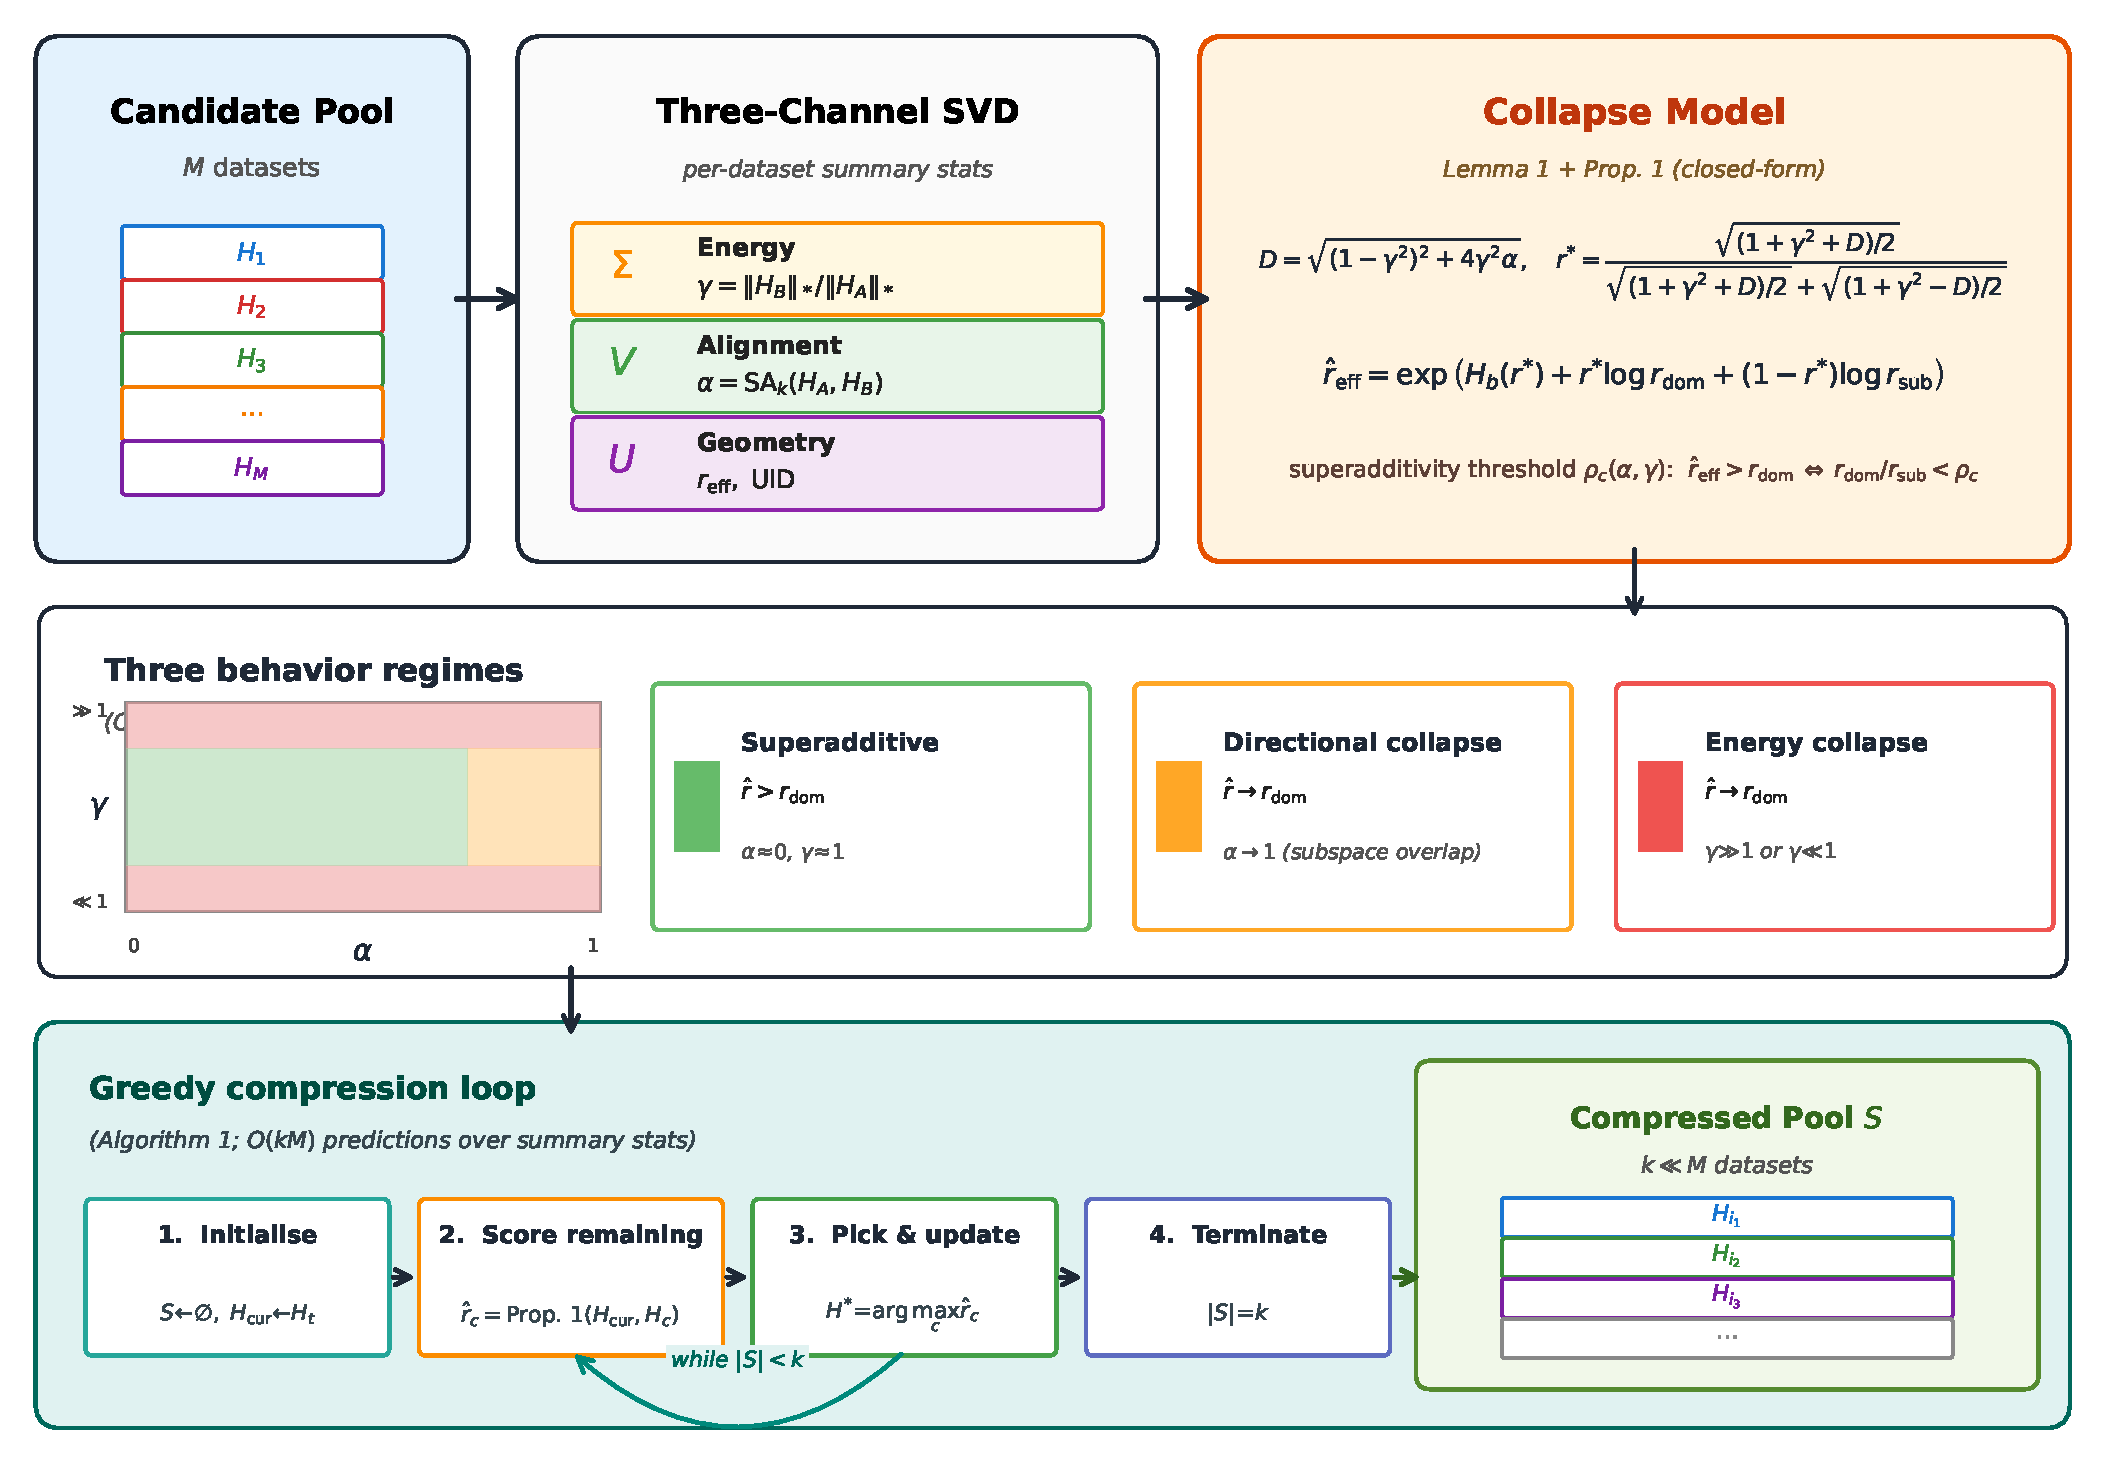
\includegraphics[width=0.88\linewidth]{fig_framework.pdf}
\caption{谱机制与选择抽象。\textbf{上部/中部：}成对方向特例与 Collapse-4S 诊断；这些面板解释局部行为，但不构成一般保证。\textbf{下部：}共同的 greedy 循环。主选择器通过组合 rank-$L$ PSD 因子为该循环评分；Collapse-4S 仅作为消融。}
\label{fig:framework}
\end{figure}

\textbf{为什么使用摘要筛选？}
穷举搜索需要 $\binom{M}{k}$ 次合并分解，并同时访问全部样本特征。Collapse-Gram-$L$ 只需 $O(kM)$ 次候选评分，每个来源传输 $O(Ld)$ 个数和三个尾部统计量。协调端无需重建原始样本特征，但这种压缩本身不构成差分隐私保证。

\textbf{贡献。}
(1)~\emph{精确代数与信息极限}：给出无条件 Gram 表示、块兼容条件下的精确分解，以及低维可识别性失败的显式反例（命题~\ref{prop:gram_general}--\ref{prop:insufficient}）。
(2)~\emph{可认证压缩}：给出可组合 rank-$L$ PSD sketch、依赖尾部的 log-effective-rank 区间，以及与单步 Full-Gram greedy 一致的充分证书（定理~\ref{thm:rank_l_bound}，推论~\ref{cor:rank_l_choice}）。
(3)~\emph{经审计的两阶段协议}：采用标签盲第一阶段抽样、明确的等来源权重、目标隔离的第二阶段评估、matched overlap 诊断、与来源无关的对照及带 provenance 校验的恢复语义（第~\ref{sec:compression} 节）。

\textbf{经验范围。}
现有成对实验评估的是 Collapse-4S，而不是新的 rank-$L$ 保证。它们在已评估样本对上表现出较强排序相关性，但相对 $r_A{+}r_B$ 的 Spearman 增量仅为 $0.003$，且校准依赖编码器。历史数据池实验也表明，不同谱方法在干净池中常选择相似子集。因此本文仅把这些结果作为有边界的证据，不能将旧表视为定理~\ref{thm:rank_l_bound} 的验证。
% ============================================================
\section{谱背景}
\label{sec:background}

对于任何特征矩阵 $H\in\R^{N\times d}$，其薄奇异值分解为 $H=U\Sigma V^\top$（$U\in\R^{N\times r}$, $\Sigma=\mathrm{diag}(\sigma_1\geq\cdots\geq\sigma_r>0)$,
$V\in\R^{d\times r}$），该分解分离出三种正交的表示方面。

\textbf{$\Sigma$ 通道 --- 谱能量。}
\textbf{有效秩} 总结了谱分布：
\begin{equation}
  \reff(H) = \exp\!\left(-\sum_{i=1}^r p_i \log p_i\right),
  \quad p_i = \frac{\sigma_i}{\sum_j \sigma_j},
  \label{eq:reff}
\end{equation}
其中 $p_i$ 是奇异值份额（未平方），因此 $r_{\mathrm{eff}}\in[1,r]$。
核范数 $\|H\|_*=\sum_i\sigma_i$ 捕捉总能量。
所有数值结果仅保留满足
$\sigma_i>\sigma_1\sqrt{8\epsilon_{64}\max(N,d)}$ 的奇异模态。
直接 SVD 与 Gram 特征值分解路径在计算核范数和有效秩前使用同一截断。
\textbf{$V$ 通道 --- 方向结构。}
右奇异向量 $V$ 编码了哪些方向被激活。
\begin{definition}[子空间对齐度]
\label{def:sa}
令 $\hat{V}_A^k,\hat{V}_B^k\in\R^{d\times k}$ 是 $H_A,H_B$ 的前 $k$ 个右奇异向量。
在级别 $k$ 的 \textbf{子空间对齐度} 定义为：
\begin{equation}
  \SAk(H_A,H_B) = \frac{1}{k}\norm{\hat{V}_A^{k\top}\hat{V}_B^k}_F^2
  = \frac{1}{k}\sum_{i=1}^k\cos^2\theta_i,
  \label{eq:sak}
\end{equation}
其中 $\theta_1\leq\cdots\leq\theta_k$ 是主角度。
\end{definition}
$\SAk\in[0,1]$: $\SAk=0$ 表示完美正交子空间（最大互补性）；
$\SAk=1$ 表示相同子空间（合并后没有新方向）。

\textbf{$U$ 通道 --- 样本几何。}
左奇异向量 $U\in\R^{N\times r}$ 编码了样本的几何分布。
通过最近邻估计的 \textbf{U 空间固有维度 (\UID)}:
\begin{equation}
  \mathrm{UID}(H) = \frac{1}{\log 2\cdot\mathbb{E}[\log(\mu_2/\mu_1)]},
  \label{eq:uid}
\end{equation}
其中 $\mu_1,\mu_2$ 是单位球体 $S^{k-1}$ 上最近邻和次近邻的测地线距离（L2 正则化后的 $U_k$ 行）。

\textbf{每个通道的作用。}
$\gamma$ 和 $\alpha$ 进入合并秩预测公式
(第 \ref{sec:method} 节) 并驱动压缩算法。
\UID 描述了单个数据集的内在几何结构
并在编码器诊断 (第 \ref{sec:e1d} 节) 中使用，但
并不出现在预测公式中；它在此处包括以完成表示空间的正交分解。

\textbf{独立性。}
成对 Spearman 检验（Bonferroni 校正，$n{=}15$ 个探针）在 ResNet-50 或
ViT-B/16 上检测到三个通道之间没有显著相关性 (所有 $p_{\mathrm{Bonf}}{>}0.38$)，这与
$\gamma,\alpha,\UID$ 捕捉了不同的属性一致。
% ============================================================
\section{塌陷模型}
\label{sec:method}

\subsection{设置与符号表示}
\label{sec:setup}

令 $H_A\in\R^{N_A\times d}$ 和 $H_B\in\R^{N_B\times d}$ 为 L2 行归一化的特征矩阵，其有效秩分别为 $r_A=\reff(H_A)$, $r_B=\reff(H_B)$，核范数分别为 $\|H_A\|_*$, $\|H_B\|_*$，子空间对齐度为 $\alpha=\SAk(H_A,H_B)$。定义：
\begin{equation}
  \gamma = \frac{\|H_B\|_*}{\|H_A\|_*} \in (0,\infty),
  \quad
  r_{\mathrm{dom}} = \begin{cases}r_A & \gamma\leq1 \\ r_B & \gamma>1\end{cases},
  \quad
  r_{\mathrm{sub}} = \begin{cases}r_B & \gamma\leq1 \\ r_A & \gamma>1\end{cases}.
\end{equation}
$\gamma$ 是这两个矩阵的 \textbf{能量比}；$r_{\mathrm{dom}}$ 是高能矩阵的有效秩。

所有来源预处理必须在子集选择前固定。对含 $N_j$ 行的来源 $j$ 声明总来源权重
$\beta_j>0$，并以 $X_j=\sqrt{\beta_j/N_j}\,H_j$ 参与后续计算。
当来源大小不同时，本文默认 $\beta_j=1$（每个来源总质量相同）；
$\beta_j=N_j$ 是另行声明的逐样本等权方案。有效秩虽然对共同缩放不变，
但对来源间相对权重的改变并不保持不变。

\subsection{主要结果}
\label{sec:theorem}

我们的分析分离了三个不能混淆的层次：无条件的格朗日恒等式、在显式解耦假设下的精确成对方向模型以及一般谱的低维摘要预测器。

\begin{proposition}[精确的格朗日表示]
\label{prop:gram_general}
令 $H_A=U_A\Sigma_A V_A^\top$ 和
$H_B=U_B\Sigma_B V_B^\top$ 为紧奇异值分解，将 $V_A$ 完成到一个正交基 $Q_A=[V_A\;V_{A,\perp}]$。用
$C=Q_A^\top V_B$ 和 $\widetilde\Sigma_A^2$ 表示 $\Sigma_A^2$ 填充零以达到维度 $d$，合并的格朗日算子满足
\begin{equation}
 Q_A^\top(H_A^\top H_A+H_B^\top H_B)Q_A
 =\widetilde\Sigma_A^2+C\Sigma_B^2C^\top.
 \label{eq:general_gram}
\end{equation}
因此，合并的奇异值是右侧特征值的平方根。
\end{proposition}

方程~\eqref{eq:general_gram} 是无条件的。一般情况下 $C$ 是稠密的：一个矩阵的一个奇异方向可以耦合到另一个矩阵的多个方向。单独的谱和平均主角统计量因此不能决定合并后的谱。
\begin{lemma}[Exact: 2$\times$2 Gram Block Eigenstructure]
\label{lem:gram}
假设成对且解耦的方向：对于每个 $i$，$V_{B,i}=\cos\theta_i V_{A,i}+\sin\theta_i V_{\perp,i}$，其中两个二维平面 $\mathrm{span}\{V_{A,i},V_{\perp,i}\}$ 互为正交。定义 \emph{模式-wise} 能量比 $\gamma_i=\sigma_{B,i}/\sigma_{A,i}$ 和 $\alpha_i=\cos^2\theta_i$。第 $i$ 个 Gram 块的特征值
\begin{equation}
 \lambda_{\pm,i}=\frac{\sigma_{A,i}^2}{2}
 \left(A_i\pm D_i\right),\quad
 A_i=1+\gamma_i^2,\quad
 D_i=\sqrt{(1-\gamma_i^2)^2+4\gamma_i^2\alpha_i}.
  \label{eq:discriminant}
\end{equation}
对应的奇异值为 $\sqrt{\lambda_{+,i}}$ 和 $\sqrt{\lambda_{-,i}}$。在所述配对和解耦条件下，此结果是精确的（附录~\ref{app:proof_thm})。
\end{lemma}

全局比值 $\gamma=\|H_B\|_*/\|H_A\|_*$ 并不意味着 $\gamma_i=\gamma$。用集合 $\{\gamma_i,\alpha_i\}$ 替换为全局摘要 $(\gamma,\alpha)$ 是一个近似步骤。

\begin{proposition}[精确比例谱模型]
\label{prop:proportional}
在引理~\ref{lem:gram} 下，进一步假设对于每个 $i$ 有 $\sigma_{B,i}=\gamma\sigma_{A,i}$ 和 $\alpha_i=\alpha$。令 $A=1+\gamma^2$, $D=\sqrt{(1-\gamma^2)^2+4\gamma^2\alpha}$，并
\begin{equation}
 q = \frac{\sqrt{(A+D)/2}}
 {\sqrt{(A+D)/2}+\sqrt{(A-D)/2}}.
  \label{eq:rstar}
\end{equation}
则合并谱由 $H_A$ 的两个缩放副本组成，并且
\begin{equation}
 r_{\mathrm{merged}}=r_A\exp(H_b(q)),\qquad r_A=r_B.
 \label{eq:proportional_exact}
\end{equation}
\end{proposition}

\begin{definition}[塌陷摘要预测器]
\label{def:collapse}
对于一般谱，我们将模式-wise 量压缩为全局核范比 $\gamma$ 和平均最高 $k$ 对齐度 $\alpha$，计算 $q$ 来自式~\eqref{eq:rstar}，并定义
\begin{equation}
  \hat{r}_{\mathrm{merged}} =
  \exp\!\Big(H_b(q) + q\log r_{\mathrm{dom}} + (1-q)\log r_{\mathrm{sub}}\Big),
  \label{eq:pred}
\end{equation}
其中 $H_b(p)=-p\log p-(1-p)\log(1-p)$。
\end{definition}
Equation~\eqref{eq:pred} 是一个基于理论的低维近似，而不是恒等式或普遍有界的估计器。它插值输入谱熵并加上理想化的两分支分裂的二元熵。其在一般谱上的准确性是一个经验问题，在 Sec.~\ref{sec:experiments} 中评估。

\textbf{解释。}
Equation~\eqref{eq:pred} 是个体秩加权对数几何平均值加上一个平衡奖金 $H_b(q)$（当 $q{=}0.5$ 时最大，随着 $q{\to}0,1$ 而消失）。

\textbf{行为模式。}
\emph{方向互补}（$\alpha{\approx}0$，$\gamma{\approx}1$）：$q{\approx}0.5$，且
$\hat{r}_{\mathrm{merged}}{\approx}2\sqrt{r_Ar_B}$。
在严格的 $(\alpha,\gamma)=(0,1)$ 情形下，该预测超加当且仅当
$r_{\mathrm{dom}}/r_{\mathrm{sub}}<4$。
\emph{方向塌陷} ($\alpha{\to}1$): $q{\to}1$, $H_b(q){\to}0$, $\hat{r}_{\mathrm{merged}}{\to}r_{\mathrm{dom}}$。
\emph{能量塌陷} ($\gamma{\gg}1$ 或 $\gamma{\ll}1$): $q{\to}1$, $\hat{r}_{\mathrm{merged}}{\to}r_{\mathrm{dom}}$。
当 $\alpha{\to}1$ \emph{和} $\gamma{\gg}1$ 时，合并的秩可以 \emph{低于} $r_{\mathrm{sub}}$——净损失多样性。

\subsection{超加性阈值}
\label{sec:superadd}

\begin{corollary}[摘要-模型超加性诊断]
\label{cor:superadd}
Equation~\eqref{eq:pred} 中的摘要预测器在 $q<1$ 时预测
$\hat{r}_{\mathrm{merged}}>r_{\mathrm{dom}}$
当且仅当
\begin{equation}
  \frac{r_{\mathrm{dom}}}{r_{\mathrm{sub}}} < \rho_c(\alpha,\gamma)
  \;\equiv\; \exp\!\!\left(\frac{H_b(q)}{1-q}\right),
  \label{eq:rho_c}
\end{equation}
其中 $q$ 来自 Equation~\eqref{eq:rstar}。
阈值 $\rho_c$ 随 $\alpha$ 增加：$\rho_c\geq4.0$ 对所有 $\alpha\in[0,0.9]$ 在 $\gamma=1$ 时成立。
随着 $q\to1^{-}$，$\rho_c\to\infty$ 而预测的增益趋于零。
在退化点 $q=1$ 中，Equation~\eqref{eq:rho_c} 的除法未定义且 Equation~\eqref{eq:pred} 给出
$\hat r_{\mathrm{merged}}=r_{\mathrm{dom}}$ 精确值。
\end{corollary}
这是摘要模型以及命题~\ref{prop:proportional} 中比例谱模型的精确决策边界；
对于一般数据，它只是诊断而不是保证。
在有限精度的经验判定中，只有当预测值或实测值 $x$ 满足
$x-r_{\mathrm{dom}}>10^{-10}\max(x,r_{\mathrm{dom}},1)$ 时才判为超加性，
从而排除等号边界上仅由舍入误差产生的正值。

\textbf{物理意义。}
$\rho_c$ 是摘要模型内部的一个决策阈值。在 $q=1$ 附近，它可以将任意小的正熵增量分类为超加性；因此 $\hat r_{\mathrm{merged}}-r_{\mathrm{dom}}$ 的大小必须与二元诊断一起报告。完全的方向重叠给出 $q=1$ 并无预测增益。证明和模型范围在附录~\ref{app:proof_thm}、\ref{app:pa_scope} 中。

\subsection{边际谱与完整主角仍不充分}
\label{sec:insufficiency}

\begin{proposition}[从边际几何无法唯一确定]
\label{prop:insufficient}
即使同时给定两个输入的边际奇异值谱和右奇异子空间之间的完整主角集合，也不能唯一确定 $\reff([H_A;H_B])$。因此，元组 $(r_A,r_B,\gamma,\alpha)$ 更不可能唯一确定它。
\end{proposition}

\textbf{反例。}
令 $e_1,e_2,e_3$ 为标准基，并构造逐行归一化矩阵
\begin{equation}
 H_A=[e_1,e_1,e_1,e_1,e_2]^\top,\quad
 H_B^{(1)}=[e_1,e_1,e_1,e_1,e_3]^\top,\quad
 H_B^{(2)}=[e_1,e_3,e_3,e_3,e_3]^\top.
\end{equation}
三者的非零奇异值均为 $(2,1)$，两组右奇异子空间的主角也均为 $\{0,\pi/2\}$；但是，两组合并 Gram 谱分别为 $(8,1,1)$ 与 $(5,4,1)$，相应有效秩为 $2.626012$ 与 $2.849536$。因此，即便完整边际谱和主角也会丢失谱质量与耦合方向的对应关系；四标量摘要丢失的信息只会更多。
\hfill$\square$

\subsection{可组合的 Rank-$L$ Gram Sketch}
\label{sec:rank_l}

上述反例说明，应直接近似 PSD 算子，而不是继续压缩为平均角度。对每个预加权来源的紧致 SVD，定义
\begin{equation}
 B_j=\Sigma_{j,1:L}V_{j,1:L}^{\top},\qquad
 \widetilde G_j=B_j^\top B_j,\qquad
 E_j=G_j-\widetilde G_j\succeq0 .
 \label{eq:rank_l_sketch}
\end{equation}
随摘要附加尾部统计量
$\tau_j=\operatorname{tr}\sqrt{E_j}$、
$\omega_j=\operatorname{tr}(E_j)$ 和
$u_j=\operatorname{rank}(E_j)$；也可使用它们的可认证上界。对集合 $S$，将因子纵向堆叠为 $B_S$，于是 $\widetilde G_S=B_S^\top B_S$，其非零谱可由较小核心 $B_SB_S^\top$ 得到，无需重建样本特征。

对 PSD 矩阵 $G$，记
$\mathcal R(G)=\exp\mathcal H(\sqrt{\lambda(G)}/\operatorname{tr}\sqrt G)$，因此 $\mathcal R(H^\top H)=\reff(H)$。定义
\begin{equation}
 T_S=\min\!\left\{\sum_{j\in S}\tau_j,
 \sqrt{\min(d,\sum_{j\in S}u_j)\sum_{j\in S}\omega_j}\right\},
 \quad
 \varepsilon_S=\frac{T_S}{\operatorname{tr}\sqrt{\widetilde G_S}+T_S}.
 \label{eq:tail_bound}
\end{equation}

\begin{theorem}[Rank-$L$ 对数有效秩误差界]
\label{thm:rank_l_bound}
假设 $\widetilde G_S\neq0$，并令
$D_S=\min(d,\sum_{j\in S}\operatorname{rank}(G_j))$。当 $D\ge2$ 时定义
\begin{equation}
 \Phi_D(\varepsilon)=
 \begin{cases}
 h_b(\varepsilon)+\varepsilon\log(D-1),
 &0\leq\varepsilon\leq1-1/D,\\
 \log D,&1-1/D<\varepsilon\leq1.
 \end{cases}
\end{equation}
则无需块兼容假设，均有
\begin{equation}
 \left|\log\mathcal R(G_S)-\log\mathcal R(\widetilde G_S)\right|
 \leq \Phi_{D_S}(\varepsilon_S).
 \label{eq:rank_l_bound}
\end{equation}
当 $D_S=1$ 时误差为零。
\end{theorem}

\begin{corollary}[单步 Full-Gram 选择证书]
\label{cor:rank_l_choice}
在某一 greedy 轮次，令
$\widehat F_j=\log\mathcal R(\widetilde G_{S\cup\{j\}})$ 且
$e_j=\Phi_{D_{S\cup\{j\}}}(\varepsilon_{S\cup\{j\}})$。若候选 $j^*$ 满足
\begin{equation}
 \widehat F_{j^*}-e_{j^*}>
 \max_{j\neq j^*}(\widehat F_j+e_j),
 \label{eq:rank_l_certificate}
\end{equation}
则 $j^*$ 是该轮精确 Full-Gram 分数的唯一最大者。
\end{corollary}

区间必须累计当前已选集合与候选的全部尾部；只使用候选自身尾部会产生错误证书。若区间不分离，应增大 $L$ 或回退到 Full-Gram。该证书只针对 greedy 的单个步骤：有效秩目标一般既非单调也非次模，因此不保证最终子集全局最优。

\textbf{旧 Collapse-4S 校准。}
在已评估真实样本对上，式~\eqref{eq:pred} 存在系统性高估。拟合乘法常数可以降低平均尺度误差；关系 $c{=}0.946{-}0.175\log(N/\reff)$ 只是已评估编码器上的经验拟合，不是普适规律。
% ============================================================
\section{旧四摘要预测器的评估}
\label{sec:experiments}

本节报告 Collapse-4S 的历史评估。这些实验检验式~\eqref{eq:pred}，并不检验 rank-$L$ 近似或其证书。证据分为三步：
(i) \textbf{理想化模型一致性}——预测器与其摘要假设下的数据一致 (§\ref{sec:e1a_main}，合成网格);
(ii) \textbf{真实数据的预测有效性}——公式在5种编码器家族、14个视觉数据集和19个文本语料库中仍然是一个强大的近似（§\ref{sec:e1d}，共427对）;
(iii) \textbf{行为模式一致性}——经验上的超加性模式与Corollary~\ref{cor:superadd}预测的三种模式一致 (§\ref{sec:e1d}，表~\ref{tab:e1d})。
这些测试用于定位启发式的有效与失效区间。额外控制见附录~\ref{app:exp_extras}。
真实数据特征矩阵进行 L2 行归一化并子采样到 $N_{\mathrm{sub}}$ 个样本；
有效秩使用公式~\eqref{eq:reff}；Bootstrap 置信区间使用 $B=10{,}000$ 次抽样。
E1a 是明确的例外：它使用未做行归一化的精确 float64 矩阵，因为行归一化会改变待核查的比例谱。

\subsection{步骤 1 --- 理想化模型一致性：合成控制网格 (E1a, 280对)}
\label{sec:e1a_main}

作为模型内一致性检查，我们在比例谱、成对方向模型下生成的 280 个受控合成对上评估 Collapse-4S（$\alpha\in\{0,0.05,0.1,0.2,0.4,0.6,0.8,1.0\}$，$\gamma\in\{0.1,0.33,0.5,1.0,2.0,3.0,10.0\}$，$d{=}512$，$N{=}1000$，每种设置重复 5 次）。

\begin{table}[t]
\centering
\caption{E1a：在精确合成网格上用直接 SVD 交叉核查唯一的 Collapse-4S 实现（$N=280$）。}
\label{tab:e1a}
\begin{tabular}{lcccc}
\toprule
方法 & $R^2$ & 最大误差 & 超加性 (\%) & $\alpha<1$ 超加性 \\
\midrule
\textbf{唯一 Collapse-4S 实现} & \textbf{1.0000} & \textbf{$1.3{\times}10^{-13}$} & \textbf{87.5\%} & \textbf{100\%} (245/245) \\
\bottomrule
\end{tabular}
\end{table}
表~\ref{tab:e1a} 显示，相对直接 SVD 的 $R^2{=}1.0000$，最大有效秩绝对误差为 $1.3{\times}10^{-13}$。
在 $\alpha{<}1$ 的 245 种配置中，超加性比例均为 100\%；全部 35 个非超加性样例只出现在 $\alpha{=}1$（子空间相同）处，验证了推论~\ref{cor:superadd} 的退化边界。
$(\alpha,\gamma)$ 热图和超加性区域的可视化见附录~\ref{app:exp_extras}。

\subsection{步骤 2--3：真实数据泛化与行为区间一致性（E1d，427 对）}
\label{sec:e1d}

接下来，我们验证该公式能否推广到其合成推导范围之外，以及它所预测的三种行为区间能否在实验中观察到。
评估覆盖 5 个编码器家族（ResNet-50、ViT-B/16、CLIP ViT-B/32、DINO ViT-S/16、SBERT）、14 个视觉数据集（CIFAR-10/100、STL-10、SVHN、MNIST、Fashion-MNIST、BloodMNIST、DermaMNIST、PathMNIST，以及 5 个 ImageNet 语义子集 \emph{animal/vehicle/artifact/food/scene}）和 19 个 SBERT 文本语料库。
总计 \textbf{427 对}（ResNet-50 为 91 对，ViT-B/16、CLIP 和 DINO 各 55 对，SBERT 为 171 对）。

\begin{table}[h]
\centering
\caption{E1d：Collapse-4S 历史关联性研究（427 对，5 个探针）。$c$ 按编码器家族分别拟合，因此校准 $R^2$ 只是描述性统计。}
\label{tab:e1d}
\small
\setlength{\tabcolsep}{3.5pt}
\begin{tabular}{lccccc}
\toprule
Probe & $n$ & Superadd.\  \% & Pearson $r$ & $c$ & $R^2_{\mathrm{cal}}$ \\
\midrule
ResNet-50 (14 datasets)       & 91  & \textbf{100\%}   & 0.940 & 0.776 & 0.760 \\
ViT-B/16 (11 datasets)        & 55  & 69.1\%            & 0.898 & 0.647 & 0.487 \\
CLIP ViT-B/32 (11 datasets)    & 55  & 29.1\%            & 0.950 & 0.595 & 0.839 \\
DINO ViT-S/16 (11 datasets)    & 55  & 36.4\%            & 0.913 & 0.584 & 0.554 \\
\midrule
\textbf{Vision (all probes)}   & \textbf{256} & \textbf{64.5\%} & \textbf{0.965} & \emph{per-probe} & \textbf{0.942} \\
+ SBERT text (19 corpora)      & +171 (427)   & 78.2\%           & 0.970          & \emph{per-probe} & 0.952 \\
\bottomrule
\end{tabular}\normalsize
\end{table}
\textbf{泛化（步骤 2）。}
该公式在全部 427 对真实数据上仍是较强的近似：未校准的总体 Pearson $r{=}0.970$，按编码器家族校准后 $R^2_{\mathrm{cal}}{=}0.952$（散点图见附录~\ref{app:exp_extras} 的图~\ref{fig:hero_scatter}）。
这表明，由理想化成对方向模型启发的摘要预测在监督 CNN、ViT、对比学习/自蒸馏 Transformer 和句子编码器等真实编码器上仍具有预测能力。

\textbf{行为区间一致性（步骤 3）。}
(i)~\textbf{ResNet-50 在 91 对数据上达到 100\% 超加性}（包括医学数据和 ImageNet），验证了推论~\ref{cor:superadd} 所预测的平衡 $(\gamma,\alpha)$ 区间。
(ii)~模型的方向重叠区间呈现出\textbf{监督/自监督分界}：CLIP 和 DINO 的超加性比例仅为 29\%--36\%，失败样例\emph{全部}集中在跨域数据对中（手写$\times$ImageNet、自然图像$\times$数字均失败），而域内数据对几乎全部成功。
双峰主角分布与极端条件数 $\kappa{\in}[10^4,10^6]$ 和这些失败相关（图~\ref{fig:bimodal_structure}）。该模式与第~\ref{sec:superadd} 节的\emph{方向塌陷}诊断一致，但并非因果识别。

\begin{figure}[t]
\centering
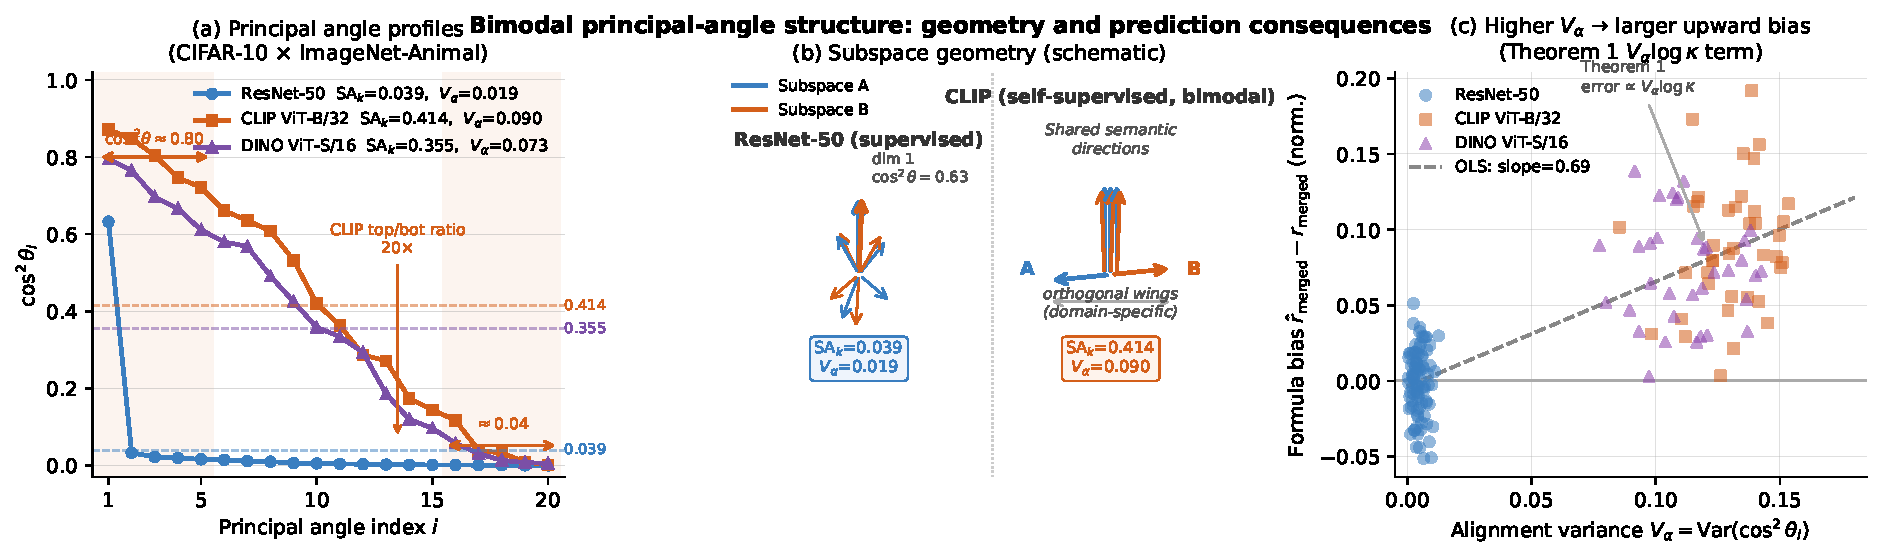
\includegraphics[width=0.97\linewidth]{fig_bimodal_structure.pdf}
\caption{\textbf{Bimodal principal-angle structure} (CIFAR-10\,$\times$\,ImageNet-Animal, $k{=}20$).
\textbf{(a)}~Per-dimension $\cos^2\theta_i$: ResNet-50 ($\SAk{=}0.039$, $V_\alpha{=}0.019$) decays monotonically from one dominant direction; CLIP ($\SAk{=}0.414$, $V_\alpha{=}0.090$) and DINO ($\SAk{=}0.355$, $V_\alpha{=}0.073$) form a two-cluster step (top-5 ratios $20{\times}$/$31{\times}$ over bot-5), violating the uniform-$\alpha$ assumption.
\textbf{(b)}~Geometric interpretation: one shared spine plus orthogonal domain-specific wings.
\textbf{(c)}~Alignment variance $V_\alpha$ predicts upward formula bias across 166 pairs (OLS slope 0.69), identifying alignment heterogeneity as an empirical failure indicator.}
\label{fig:bimodal_structure}
\end{figure}
\paragraph{量化双模态差距。}
每个探针校准后的 $R^2$: CLIP $0.84>$ ResNet $0.76>$ DINO $0.55>$ ViT $0.49$;
在四个视觉探针上相关系数均不低于 $0.90$，但这不构成一般准确性保证。
Figure~\ref{fig:bimodal_structure}(a,c) 显示了 CLIP/DINO 的双聚类 $\cos^2\theta_i$ 分布 ($V_\alpha > 0.07$)，放大了观察到的预测偏差，识别出与全局摘要近似相比的具体偏离而非黑盒失败（完整机制见附录~\ref{app:bimodal})。

(iii) \textbf{能量塌陷} 出现在 ViT 的 17 对非超加性成对方向中，所有这些都在 $\gamma \notin [0.5,2]$ 中，与摘要模型的能量不平衡诊断一致。
(iv) \textbf{跨模态检查}: 在 171 个 SBERT 文本样本对上，排序相关降至 $r=0.793$（98.8\% 超加性），因此数据不支持模态无关主张。视觉侧拟合关系只能解释 $R^2=0.08$ 的 SBERT 方差，说明必须单独验证文本编码器。

\textbf{评估总结。}
步骤 1--3 只建立模型内一致性、当前基准上的关联性与可观察的定性模式。它们既不验证 Collapse-Gram-$L$，也不建立普适精确性：命题~\ref{prop:insufficient} 已证明四摘要通常无法确定合并秩。
跨数据集校准泛化、跨探针一致性及 $\reff$/LP-准确率对应关系 ($\rho = 0.90$ 在 ViT 家族内) 见附录~\ref{app:exp_extras}。

% ============================================================
\section{两阶段数据池压缩}
\label{sec:applications}
\label{sec:compression}
\label{sec:pool_selection}

第一阶段的目标是生成标签盲短名单，而不是直接作出最终效用决策。Collapse-Gram-$L$ 将第~\ref{sec:rank_l} 节的可组合 sketch 用于算法~\ref{alg:collapse_greedy}。在当前第二阶段审计中，每个候选 adapter 都使用该来源的标签训练；目标 train 内部的 repeated cross-validation 拟合 ridge probe 并选择来源。目标 test 只在选择冻结后打开。这是“来源监督适配 + 目标验证选择”，不是在目标数据上训练 adapter。之所以必须分层，是因为谱多样性本身不能决定任意目标任务的效用。

\paragraph{修正后的协议。}
第一阶段在不读取标签的情况下抽取来源样本；大小不同的来源使用预先声明的等来源权重 $X_j=H_j/\sqrt{N_j}$（$\beta_j=1$）。对比方法包括 Collapse-Gram-$L$、rank-only、DPP、Facility Location、凝聚式 medoid、leverage-score、随机选择和 Full-Gram greedy；只有组合数不超过预先声明的门限时，才加入合并秩的穷举 oracle。第二阶段为所有候选分配相同的来源监督优化步数和随机种子，并加入 frozen-identity 与未训练 random-adapter 对照。选择前唯一允许的目标信号是目标 train 内部的交叉验证，所有 adapter checkpoint 均保存哈希；选择 manifest 写入并冻结后，独立 held-out 命令才允许打开目标 test 缓存。运行清单用 SHA-256 绑定代码、输入、预处理、权重、采样索引、checkpoint 和超参数；不完整的 source/seed 组不能作为已完成结果恢复。重叠检测使用同数据集 matched negatives，且 $0\%$ 重叠条件不存在真实 parent。为估计所有 shortlist 的穷举 regret，本次审计离线训练了全部候选 adapter，因此其总墙钟并不是已实测的部署节省。

\paragraph{经审计的历史 pilot。}
修正前的 21 来源 pilot 使用按标签分层的来源缓存，在选择冻结前查询目标 test，且没有评估 Collapse-Gram-$L$。其中 DPP 与 rank-only 的 Recall@10 都为 $85.71\%$，并对近似平局高度敏感；本文只将它保留为历史审计基线，以下报告修正版结果。

\paragraph{修正版受控证据。}
中间版本 \texttt{corrected\_v2} 因统计定义不一致和 provenance 不完整而作废。在替代的 \texttt{corrected\_v3} 扫描中，4 个编码器、10 个构造种子、6 个重叠率和 4 个预算在每个 rank 下形成 960 个配置。表~\ref{tab:v3_rank_sweep} 报告编码器宏平均。每个选中前缀区间都包含精确分数，但所有被评估决策的候选区间均重叠：该界有效，却在这些 rank 下没有实际决策力。DPP 在这个受控谱保持任务中更强；这只是记录了实际但不相等的通信成本，不能视作等字节 Pareto 结论。

单独的 $L=20$ 精确参照（4 个编码器、3 个种子、288 个配置、Random-100）中，rank-$L$/DPP/Full-Gram 相对 rank-only 的增益分别为 $3.65/5.37/5.81\%$。其区间覆盖 $288/288$ 个前缀，但仅认证 $0/720$ 步，并与 Full-Gram 有序前缀完全一致 $0/288$ 次；这里的 Full-Gram 只是 greedy 参照，不是全局 oracle。

\begin{table}[t]
\centering
\caption{修正版受控 rank 扫描。增益是相对 rank-only 的最终精确合并有效秩。每行 960 个选中前缀区间全部覆盖精确分数。}
\label{tab:v3_rank_sweep}
\small
\setlength{\tabcolsep}{3.2pt}
\begin{tabular}{crrrr}
\toprule
$L$ & Gram 增益 & DPP 增益 & 平均误差/上界 & 已认证步骤 \\
\midrule
10 & $+2.09\%$ & $+4.90\%$ & $2.558/5.944$ & $0/2{,}400$ \\
20 & $+3.81\%$ & $+5.48\%$ & $1.877/5.505$ & $0/2{,}400$ \\
50 & $+4.94\%$ & $+5.68\%$ & $0.996/4.455$ & $0/2{,}400$ \\
\bottomrule
\end{tabular}\normalsize
\end{table}

\paragraph{修正版 held-out 效用证据。}
自然池复算包含 21 个来源、7 个目标、4 个编码器和 5 个 adapter seeds。在短名单 $10/21$ 下，rank-$L$、rank-only、DPP 与 Full-Gram greedy 的严格 oracle recall 分别为 $75.00\%$、$85.71\%$、$85.71\%$ 和 $89.29\%$，均未达到预先声明的 $90\%$ 门槛。它们在 adapter 族内部的 held-out regret 很小（$0.00022$--$0.00082$），但该 adapter 族没有通过来源无关对照。frozen identity、未训练 random adapter 和验证 oracle 来源监督 adapter 的平均 held-out 准确率分别为 $0.83654$、$0.77144$ 和 $0.76951$。oracle 减 identity 为 $-0.06703$（target-cluster 95\% CI $[-0.09771,-0.04400]$）；所有确定性方法选出的 adapter 在 28 个 encoder-target 单元中都低于 identity。因此，小 regret 不能解释为效用得到保留或来源数据有益。

\paragraph{解释。}
理论只控制谱分数的近似误差。修正版扫描确认了区间覆盖，却也表明覆盖本身未必产生可用的决策证书。第二阶段随后在任何实际压缩主张之前否决了当前来源监督 adapter 族。因此，严格候选身份、允许平局的 recall、regret 和来源无关效用对照必须分别报告。

\section{结论}
\label{sec:conclusion}

本文将精确谱结构、有界近似与任务相关证据分开。Gram 可加性和块兼容局部模型是精确结论；反例则排除了从旧摘要作普适预测的可能。rank-$L$ sketch 具有有效的确定性误差区间，但修正版扫描在 $L\leq50$ 时得到零个决策证书，并发现 DPP 至少同样有竞争力。held-out 审计的结论更为明确：即使验证 oracle 的来源监督 adapter 也显著差于 frozen identity。因此，本文当前的贡献是精确局部分析、可审计的近似协议和有记录的负面结果，而不是已经验证的实际压缩器。正面的应用主张至少需要等字节 Pareto 证据，以及一个首先能够超过 identity 的下游 adapter 族。
代码可在\url{https://anonymous.4open.science/r/collapsemodel-1DB6} 获取。

\bibliographystyle{abbrvnat}
\bibliography{references}

% ============================================================
\appendix

\section{局限性}
\label{app:limitations}

四摘要 $(r_A,r_B,\gamma,\alpha)$ 一般不足以确定合并有效秩（命题~\ref{prop:insufficient}）。精确 $2\times2$ 分解需要逐模态配对与解耦，闭式熵表达还要求比例谱和均匀对齐；Collapse-4S 因而没有普适误差界。经验校准关系只在少量编码器上拟合，并且对 SBERT 转移较差。rank-$L$ 定理要求在固定、与子集无关的预处理下使用精确 PSD 截断或合法尾部上界；依赖所选集合的全局中心化会破坏直接可组合性。当前区间在 $L\leq50$ 时宽到无法认证任何已测选择，增大 $L$ 又会提高通信量；现有基线也没有做到等字节匹配。形成 Gram 矩阵还会平方条件数，所以极端病态输入需要用直接 SVD 交叉检查或加入明确的数值余量。最后，无标签几何无法决定任意标签。修正版自然池仍然领域不均衡，来源监督 bottleneck adapter 也是一个未能超过 frozen identity 的窄代理。因而 LoRA 与多池训练已按预注册停止规则不再执行；只有覆盖更多独立域并先找到有效的 adapter 族，才能主张实际效用。
\section{精确格拉姆结果的证明}
\label{app:proof_thm}

\textbf{Proposition~\ref{prop:gram_general}.}
从紧凑的 SVD 中，
$H_A^\top H_A=V_A\Sigma_A^2V_A^\top$ 和
$H_B^\top H_B=V_B\Sigma_B^2V_B^\top$。
因为 $Q_A$ 的第一列是 $V_A$，
所以 $Q_A^\top V_A\Sigma_A^2V_A^\top Q_A=\widetilde\Sigma_A^2$。
设 $C=Q_A^\top V_B$，则
$Q_A^\top V_B\Sigma_B^2V_B^\top Q_A=C\Sigma_B^2C^\top$。
上述推导证明了式~\eqref{eq:general_gram}。正交相似性保持特征值，其平方根即为合并后的奇异值。$\square$

\textbf{Lemma~\ref{lem:gram}.}

在成对、解耦的方向下，$H_B$ 的第 $i$ 个右奇异向量是
$V_{B,i}=\cos\theta_i V_{A,i}+\sin\theta_i V_{\perp,i}$，
其中 $V_{A,i}$ 是 $H_A$ 的第 $i$ 个右奇异向量，且这两个二维平面相互正交。
在基 $\{V_{A,i},V_{\perp,i}\}$ 下：
\begin{align}
  H_A^\top H_A \text{ (block)} &= \sigma_{A,i}^2\begin{pmatrix}1&0\\0&0\end{pmatrix}, \\
  H_B^\top H_B \text{ (block)} &= \sigma_{B,i}^2
    \begin{pmatrix}\cos^2\theta_i & \cos\theta_i\sin\theta_i \\
    \cos\theta_i\sin\theta_i & \sin^2\theta_i\end{pmatrix}.
\end{align}
定义模式比 $\gamma_i=\sigma_{B,i}/\sigma_{A,i}$；无需全局比例谱假设。求和得到
\begin{equation}
  G_i = \sigma_{A,i}^2\begin{pmatrix}1+\gamma_i^2\alpha_i & \gamma_i\sqrt{\alpha_i(1-\alpha_i)} \\
    \gamma_i\sqrt{\alpha_i(1-\alpha_i)} & \gamma_i^2(1-\alpha_i)\end{pmatrix},
\end{equation}
其中 $\alpha_i=\cos^2\theta_i$。
其迹为 $\sigma_{A,i}^2(1+\gamma_i^2)$，行列式为
$\sigma_{A,i}^4\gamma_i^2(1-\alpha_i)$，通过二次公式得到式~\eqref{eq:discriminant}。$\square$

\textbf{Proposition~\ref{prop:proportional}.}

设 $\gamma_i=\gamma$ 且 $\alpha_i=\alpha$，定义 $c_\pm=\sqrt{(A\pm D)/2}$。引理~\ref{lem:gram} 给出了合并后的奇异值集合
$\{c_+\sigma_{A,i}\}_i\cup\{c_-\sigma_{A,i}\}_i$。
经过核范数归一化后，它们的概率分别为 $qp_i^A$ 和 $(1-q)p_i^A$，其中
$q=c_+/(c_++c_-)$。因此
\begin{align}
 H_{\mathrm{merged}}
 &=H_b(q)+qH(p^A)+(1-q)H(p^A)\\
 &=H_b(q)+\log r_A.
\end{align}
通过指数化证明了式~\eqref{eq:proportional_exact}。比例谱具有相同的归一化奇异值分布，因此 $r_A=r_B$。$\square$

\textbf{定理~\ref{thm:rank_l_bound}。}
记 $E_S=\sum_{j\in S}E_j$。对 PSD 矩阵，
$\operatorname{tr}\sqrt{A+B}\leq\operatorname{tr}\sqrt A+
\operatorname{tr}\sqrt B$，该式可由对
$[A^{1/2},B^{1/2}]$ 使用核范数三角不等式得到。因此
\begin{equation}
 \operatorname{tr}\sqrt{E_S}\leq\sum_j\tau_j,
 \qquad
 \operatorname{tr}\sqrt{E_S}
 \leq\sqrt{\operatorname{rank}(E_S)\operatorname{tr}(E_S)}
 \leq\sqrt{\min(d,\sum_j u_j)\sum_j\omega_j},
\end{equation}
从而 $\operatorname{tr}\sqrt{E_S}\leq T_S$。将
$a_i=\sqrt{\lambda_i(\widetilde G_S)}$ 与
$b_i=\sqrt{\lambda_i(G_S)}$ 按降序排列。由
$G_S\succeq\widetilde G_S$ 可知 $b_i\geq a_i$。令
$\widetilde\nu=\sum_i a_i$、$\delta=\sum_i(b_i-a_i)$，则
$0\leq\delta\leq T_S$。当 $\delta>0$ 时，真实归一化谱满足
\begin{equation}
 p=\frac{\widetilde\nu}{\widetilde\nu+\delta}\widetilde p
 +\frac{\delta}{\widetilde\nu+\delta}q,
 \qquad q_i=\frac{b_i-a_i}{\delta}.
\end{equation}
因此 $\operatorname{TV}(p,\widetilde p)\leq
\delta/(\widetilde\nu+\delta)\leq\varepsilon_S$。在至多 $D_S$ 维的支撑上应用 Fannes--Audenaert 熵连续性界，即得式~\eqref{eq:rank_l_bound}。$\delta=0$ 与 $D_S=1$ 的情况直接成立。$\square$

\textbf{推论~\ref{cor:rank_l_choice}。}
由定理，每个精确候选分数均落在
$[\widehat F_j-e_j,\widehat F_j+e_j]$ 中。式~\eqref{eq:rank_l_certificate} 使 $j^*$ 的下端点严格高于所有竞争者的上端点，故结论成立。$\square$

\textbf{Status of Eq.~\eqref{eq:pred}.}
对于非等价或不成比例的谱，两个分支不必继承输入分布，并且 $q$ 可以在模式间变化。因此，方程~\eqref{eq:pred} 定义了一个结构化的近似；并未断言其精确性或通用误差界。

\section{组合优化边界}
\label{app:optimization_limits}

有效秩最大化通常并不单调。令
$G_A=\operatorname{diag}(1/2,1/2)$、
$G_B=\operatorname{diag}(1,0)$，则
$\mathcal R(G_A)=2$，而
$\mathcal R(G_A+G_B)=1.928623<2$。
该目标通常也不满足次模性。令
$G_0=\operatorname{diag}(1/5,4/5)$、
$G_1=\operatorname{diag}(0,1)$、
$G_2=\operatorname{diag}(1,0)$。对
$A=\{0\}\subset B=\{0,1\}$，直接计算
$F(S)=\log\mathcal R(\sum_{j\in S}G_j)$ 可得
\begin{equation}
 F(A\cup\{2\})-F(A)=0.051522
 <0.125701=F(B\cup\{2\})-F(B),
\end{equation}
违反边际收益递减。因此，标准单调次模 greedy 保证不适用；穷举搜索只能作为有限小数据池上的参照。
\section{Bootstrap Confidence Intervals}
\label{app:bootstrap}

\begin{table}[h]
\centering
\caption{Bootstrap 95\% CIs ($B=10{,}000$, seed=42) for all key metrics.}
\label{tab:bootstrap_ci}
\begin{tabular}{llccc}
\toprule
实验 & 指标 & 点估计 & 95\% CI & SE \\
\midrule
E1a (280 对)  & $R^2$                  & 1.0000 & [1.0000, 1.0000] & 0.000000 \\
E1a                & 超加性 ($\alpha<1$)     & 1.0000 & [1.000, 1.000]  & 0.000000 \\
E1b (30 对)       & Pearson $r$             & 0.9478 & [0.906, 0.978]  & 0.019 \\
E1b                & 超加性 \%               & 0.8667 & [0.733, 0.967]  & 0.062 \\
E1c (57 对)       & $R^2$ (全局)            & 0.049  & [-0.346, 0.287] & 0.161 \\
E1c                & Pearson $r$ (全局)      & 0.928  & [0.894, 0.949]  & 0.014 \\
E1c                & 超加性 \%               & 0.930  & [0.860, 0.982]  & 0.034 \\
E1c (ResNet-50)   & 超加性 \%               & 1.000  & [1.000, 1.000]  & 0.000 \\
E1c (ResNet-50)   & Pearson $r$             & 0.934  & [0.885, 0.965]  & 0.021 \\
E1c (ViT-B/16)    & 超加性 \%               & 0.733  & [0.467, 0.933]  & 0.114 \\
E1c (ViT-B/16)    & Pearson $r$             & 0.945  & [0.883, 0.982]  & 0.026 \\
E1c (SBERT)       & 超加性 \%               & 1.000  & [1.000, 1.000]  & 0.000 \\
\bottomrule
\end{tabular}
\end{table}
% ============================================================
% ============================================================
\section{自监督编码器中的双模态主角结构}
\label{app:bimodal}

每个维度的 $\cos^2\theta_i$ 模式及其预测后果如图~\ref{fig:bimodal_structure}（正文）所示：CLIP/DINO 展现出两簇阶梯结构（上五分位数/下五分位数比值 $20{\times}$/$31{\times}$，$V_\alpha{=}0.090$/$0.073$），而 ResNet-50 单调递减 ($V_\alpha{=}0.019$)。

\textbf{低 $R^2$ 探针由两种不同的机制驱动。} 对于 DINO ($R^2{=}0.55$)，原因是下面分析的双模态 $\cos^2\theta_i$。对于 ViT ($R^2{=}0.49$，监督式)，原因在于 \emph{能量不平衡} 而非双模态：17/17 的 ViT 非超加性对位于 $\gamma{\notin}[0.5,2]$（跨分辨率对如 MNIST $\times$ ImageNet），其中全局能量摘要极端，两成分混合近似效果下降。ViT 的主角分布保持均匀（无双模态）；其较低的 $R^2$ 实际上标记了能量不平衡区间为可靠性边界。我们为了透明性保留完整的 ViT 行在表~\ref{tab:e1d} 中，并将 $\gamma{\in}[0.5,2]$ 标记为 ViT 可靠的应用窗口。

\textbf{诚挚的范围声明。} 我们将双模态失败模式视为当前公式的真正边界，而非特征。当主角分布呈现双模态时，全局摘要近似背后的均匀 $\alpha$ 假设被强调，并且自监督对比/蒸馏编码器（CLIP, DINO）系统地在跨域对上产生此类分布。在此范围内，校准公式仍然正确排序（所有四个探针的皮尔逊 $r{\geq}0.90$，表~\ref{tab:e1d}），但绝对预测 $\hat r$ 偏向上移且超加性决策边界被改变，解释了 CLIP/DINO 跨域对上观察到的 29--36\% 的超加性率。\textbf{崩溃模型在这里所做的贡献}在于机制化局部化：$\cos^2\theta_i$ 中双模态顶/底比值 ${>}20{\times}$（图~\ref{fig:bimodal_structure}）揭示了被标量摘要忽略的对齐异质性，而非将其失败作为黑盒惊喜。
\textbf{不奏效的方法。}
一个简单的能量加权片段
$\bar\alpha_w{=}\sum_i(\sigma_i/\|H\|_*)\cos^2\theta_i$
恶化了预测（皮尔逊 $r$ 下降 $1$--$2\%$，MAE 上升 $6$--$8\%$），因为它过度强调最对齐方向的冗余性同时抑制中间方向的贡献。

\textbf{我们认为有效的方法及其测试方法。}
自然的下一步是一个 \emph{分段成对方向模型}：
将 $k$ 个方向分为高对齐簇（$\cos^2\theta_i{\geq}\tau$）和低对齐簇，分别在每个簇内应用引理~\ref{lem:gram}，并结合结果分支谱。这比单一均值保留了更多的 $\alpha_i$ 分布，但仍需要控制谱配对和跨方向耦合。我们将在未来的工作中扩展此方法及其误差分析。

% ============================================================
\section{历史 $M{=}14$ 视觉池与 $M{=}7$ 文本池压缩 Pilot}
\label{app:compression_m14}

该实验早于标签盲缓存、来源权重和 Collapse-Gram-$L$ 实现；其中的 Collapse 均指 Collapse-4S，以下数字仅作为历史描述。

\begin{table}[h]
\centering
\caption{策略、架构和模态下的多样性保留 $\reff^{\mathrm{sel}}/\reff^{\mathrm{full}}$ (\%)。
FacLoc = 设施位置（$\SAk$ 核上的子模贪婪算法）；
$k$Medoids = $1{-}\SAk$ 距离的 PAM；随机项为10次种子的均值$\pm$标准差。该历史表只比较谱保持率，不构成任务效用保证。}
\label{tab:compression}
\small
\setlength{\tabcolsep}{2.5pt}
\begin{tabular}{llcrrrrc}
\toprule
探测器 & $M$ & $k$ (比例) & Collapse-4S & FacLoc & kMedoids & 随机 & LP$_{\mathrm{4S}}$ \\
\midrule
\multicolumn{8}{l}{\textit{视觉}} \\
ResNet-50 & 14 & 3 ($4.7{\times}$) & \textbf{101.4} & 87.8 & 87.5 & $84.3_{\pm10.0}$ & 0.754 \\
ResNet-50 & 14 & 5 ($2.8{\times}$) & \textbf{105.7} & 95.6 & 92.6 & $88.7_{\pm5.3}$ & 0.754 \\
ResNet-50 & 14 & 7 ($2.0{\times}$) & \textbf{105.9} & 98.4 & 98.0 & $93.1_{\pm7.6}$ & 0.747 \\
ViT-B/16  & 11 & 3 ($3.7{\times}$) & \textbf{103.6} & ---  & ---   & $92.0_{\pm3.3}$ & 0.779 \\
ViT-B/16  & 11 & 5 ($2.2{\times}$) & \textbf{104.9} & ---  & ---   & $94.1_{\pm3.7}$ & 0.779 \\
\midrule
\multicolumn{8}{l}{\textit{文本}} \\
BERT L6    & 7 & 3 ($2.3{\times}$) & \textbf{103.6} & ---  & ---   & $97.8_{\pm5.0}$ & --- \\
RoBERTa L6 & 7 & 3 ($2.3{\times}$) & \textbf{103.8} & ---  & ---   & $97.0_{\pm6.1}$ & --- \\
GPT-2 L6   & 7 & 3 ($2.3{\times}$) & \textbf{104.8} & ---  & ---   & $92.8_{\pm9.5}$ & --- \\
GPT-2 L6   & 7 & 5 ($1.4{\times}$) & \textbf{106.0} & ---  & ---   & $96.7_{\pm4.7}$ & --- \\
\bottomrule
\end{tabular}\normalsize
\end{table}
在该 ResNet-50 历史池中，Collapse-4S 的谱保持率比 Facility Location 高
$7.5$--$13.6$ 个百分点，比 $k$-Medoids 高 $7.9$--$13.9$ 个百分点。
配套 LP 数值来自窄范围 pilot，且未按修正后的两阶段协议产生；它们不能证明谱保持率排序会迁移到新目标。

% ============================================================
\section{$r_A{+}r_B$ 启发式方法：安全区间和失败模式}
\label{app:rsum_regime}

\paragraph{何时 $r_A{+}r_B$ 足够，何时会失效？}
在干净的历史数据池中，$r_A{+}r_B$、Max-$\reff$ 与 Collapse-4S 经常选择相同子集（在旧 $M{=}43$ 压力测试中相差不超过 $0.7$\,pp）。这只说明旧启发式在该数据区间近似退化为 rank-only，不能将单个秩称为充分统计量。
\textbf{(i)~先验低冗余度诊断。}
从每个数据集的摘要计算得到的 $\rho_c(\bar\alpha,\bar\gamma)$ \emph{表明} 在不实际运行竞争策略的情况下，$r_A{+}r_B$ 很可能达成一致。在我们的 ResNet-50 视觉池中，top-$\reff$ 对之间的 $\bar\alpha{<}0.2$ 放置 $r_{\mathrm{dom}}/r_{\mathrm{sub}}$ 在预测的一致区间内（$\rho_c{>}4$ 且 $\bar\alpha{\leq}0.2$，参见推论定理~\ref{cor:superadd})，与在 $M{=}14$ 和 $M{=}43$ 时观察到的启发式等价一致。
\textbf{(ii)~检测不安全区间。}
当候选者包含近似重复或强对齐子空间时，$\alpha$ 通道提供了 rank-only 未保留的信息。下面的克隆压力测试中，$r_A{+}r_B$ 的谱保持率下降 $25.5\%$，而 Collapse-4S 在该构造上避免了部分冗余选择。自然二模态 CLIP/DINO 跨域对（第~\ref{sec:e1d} 节，$\alpha\in[0.35,0.41]$ 且 top-5 $\cos^2\theta\geq0.7$）进一步说明对齐不可忽略，但并不直接证明任一选择器在自然池上的优势。
\textbf{(iii)~无需执行的诊断。}
Collapse-4S 的区间分类（超加性 / 方向塌陷 / 能量塌陷）可从 $(\gamma,\alpha)$ 计算，但命题~\ref{prop:insufficient} 表明它只能作为先验诊断，不能作为认证决策规则。
\paragraph{冗余克隆陷阱：$r_A{+}r_B$ 的失败模式}
为了测试摘要方法在近重复项下的行为，我们构造了一个 \emph{克隆压力测试}：池中具有最高 $\reff$ 值的数据集（STL-10，$\reff{=}994$）通过随机旋转 $H_{\mathrm{clone}}{=}H_{\mathrm{orig}}Q(\theta)$ 生成 5 个近克隆（$\theta\in\{0.01,0.03,0.05,0.07,0.10\}$，$\SAk{>}0.99$）。在包含 5 个真实 ResNet-50 数据集和 5 个克隆的池中，$k{=}3$ 时 $r_A{+}r_B$ 选择 $2/3$ 个克隆（$\reff^{\mathrm{merged}}{=}997$），Collapse-4S 未选择克隆（$\reff^{\mathrm{merged}}{=}1251$）；$k{=}5$ 时二者分别选择 $4/5$ 和 $2/5$ 个克隆（$\reff{=}998$ 与 $1233$）。该结果在五个 $\theta$ 值下保持一致。它说明对齐信息能区分 rank-only 无法区分的近重复项，但作为人为构造的压力测试，不能证明自然分布上的普适性能。

% ============================================================
\section{P2-E: 混合双信号策略}
\label{app:p2e_hybrid}

历史 $M{=}40$ pilot 提示了一个双信号混合策略：先用一种信号选择 $\lceil k/2\rceil$ 个数据集，再用另一种信号填充剩余预算。我们在同一个 ResNet-50 数据池中测试三种顺序：
\textbf{Col$\to$Cen}（先崩溃，残差上使用质心-前馈），\textbf{Cen$\to$Col}（先质心-前馈，残差上使用崩溃），以及 \textbf{Col$\to$Dom}（先崩溃，残差上使用域多样性）。
\begin{table}[h]
\centering
\caption{Two-signal hybrid strategies on $M{=}40$ ResNet-50.
Pure-strategy reference rows are shown for comparison.
\textbf{Bold} marks the best LP at each $k$.}
\label{tab:p2e_hybrid}
\small
\setlength{\tabcolsep}{4pt}
\begin{tabular}{lcccccc}
\toprule
& \multicolumn{2}{c}{$k{=}5$ ($8.0{\times}$)} & \multicolumn{2}{c}{$k{=}7$ ($5.7{\times}$)} & \multicolumn{2}{c}{$k{=}10$ ($4.0{\times}$)} \\
\cmidrule(lr){2-3}\cmidrule(lr){4-5}\cmidrule(lr){6-7}
Strategy & Ret\% & LP & Ret\% & LP & Ret\% & LP \\
\midrule
\multicolumn{7}{l}{\textit{Pure (reference)}} \\
Collapse                  & 117.2 & 0.7576 & 117.4 & 0.7578 & 116.2 & 0.7576 \\
Centroid-FF               &  93.4 & 0.7570 &  96.7 & 0.7624 & 100.5 & 0.7630 \\
DomainDiverse             & 114.7 & 0.7634 & 111.8 & 0.7596 & 113.8 & 0.7544 \\
\midrule
\multicolumn{7}{l}{\textit{Hybrid two-stage}} \\
Col$\to$Cen               & 110.2 & 0.7534 & 111.9 & 0.7496 & 113.8 & 0.7546 \\
\textbf{Cen$\to$Col}      & 106.7 & 0.7596 & 113.6 & \textbf{0.7610} & 115.0 & \textbf{0.7602} \\
Col$\to$Dom               & 114.7 & \textbf{0.7634} & 116.0 & 0.7562 & 113.8 & 0.7544 \\
\bottomrule
\end{tabular}\normalsize
\end{table}

\textbf{Cen$\to$Col 是一致的混合策略胜者。}
在 $k{\in}\{7,10\}$（操作压缩范围）下，Cen$\to$Col 实现了 LP 为 $0.7610/0.7602$，比纯 Collapse ($0.7578/0.7576$) 高出 ${+}0.0032/{+}0.0026$，同时仅牺牲了 $3.8/1.2$\,pp 的保留率。
在 $k{=}10$ 时，Cen$\to$Col 以 $1.2$ 个百分点的谱保持损失换取 $0.0026$ 的 LP 增量；它并未同时支配纯 Collapse 的两个指标。
与纯 Centroid-FF 相比，在 $k{=}5$ 时 Cen$\to$Col 恢复了 $13.3$\,pp 的保留率，在 $k{=}7$ 时恢复了 $16.9$\,pp，而在 $k{=}10$ 时恢复了 $14.5$\,pp，同时保持 LP 在 $\pm0.0028$ 内。
相比之下，\textbf{Col$\to$Cen} 却损害了两个指标：一旦 Collapse 选择了高-$\reff$ 数据集，添加“不同原型”的数据集会稀释谱而无法恢复质心覆盖。
\textbf{Col$\to$Dom} 在此池中简化为 DomainDiverse 因为 DomainDiverse 已经选择了 STL-10 和 fashion\_mnist（各自领域内高-$\reff$ 的数据集），这些数据集也是 Collapse 会选择的。
\textbf{推论。}
排序很重要：从质心-FF 开始建立了几何基础，随后 Collapse 通过高-\reff 补充了互补方向。摘要公式在这个混合策略中的作用是 \emph{填充} 剩余预算以选择最大化多样性的选项，这正是它仅使用汇总统计量运行的领域（质心-FF 前缀可以从已共享的质心中预先计算一次，无需交换特征矩阵）。
这一单池结果只提供设计动机，不能验证可组合混合策略；仍需在修正协议和独立目标上重复。

% ============================================================
\section{E5 补充材料：每个目标的选择细节}
\label{app:e5_downstream}

\textbf{每个目标的后悔表（M=10 池）。}
\begin{center}
\setlength{\tabcolsep}{5pt}
\begin{tabular}{lcccc}
\toprule
& \multicolumn{4}{c}{平均后悔率 (\%) / 平均召回率 (\%)} \\
\cmidrule(lr){2-5}
策略 & $K{=}1$ & $K{=}2$ & $K{=}3$ & $K{=}5$ \\
\midrule
Collapse-4S & \textbf{0.0 / 100} & \textbf{0.0 / 100} & \textbf{0.0 / 100} & \textbf{1.0 / 87} \\
Max-$\reff$ & 0.0 / 67 & 2.0 / 67 & 0.9 / 89 & 1.0 / 87 \\
$\Ddir$-贪婪 & 20.3 / 0 & 16.7 / 17 & 17.0 / 33 & 13.3 / 40 \\
随机选择 & 15.2 / -- & 17.5 / -- & 16.1 / -- & 11.1 / -- \\
\bottomrule
\end{tabular}
\end{center}

对于 BloodMNIST ($K{=}1$)，Max-$\reff$ 选择了 STL-10（单个 $\reff{=}357$ 最高），而 Collapse-4S 选择了 CIFAR-100（$\reff{=}356$，略低），因为后者与 BloodMNIST 的对齐度较低 ($\alpha{=}0.18$ vs.\ $0.21$)。在这一历史样例中，实际合并秩分别为 $506.8$ 和 $506.4$；差异很小，不能单独建立稳定优势。

\textbf{$r_A{+}r_B$ 贪婪基线。}
我们评估了一个 $r_A{+}r_B$ 贪婪策略，该策略在每一轮选择具有最高单个 $\reff$ 的候选者。
在 M=10 池中，此基线在 $K{\leq}3$ 时与 Collapse-4S 匹配（相同的子集，后悔率为 $0\%$），仅在 $K{=}5$ 处出现分歧，在该处 Collapse-4S 的召回率为 $100\%$，而 $r_A{+}r_B$ 为 $87\%$。
该单池结果说明两者多数情况下等价，并给出一个可能由对齐度区分的样例；它不足以划定一般失效边界。
\textbf{下游线性探针验证。}
我们在每个策略的 $K$-子集合并特征上训练一个线性探针，并在保留的测试数据上进行评估。
四种策略（穷举法、贪婪塌陷、$r_A+r_B$、最大有效秩）在所有 6 种测试配置中（CIFAR-10 和 STL-10 目标，$K{\in}\{1,2,3\}$）的线性探针准确率完全相同，
范围从 $0.776$（CIFAR-10，$K{=}3$）到 $0.979$（STL-10，$K{=}1$）。由于所有方法的 LP 完全相同，该实验不能区分选择器，也不能证明最大化有效秩改善下游效用。

% ============================================================
\section{E7 补充材料：kNN 下游验证}
\label{app:e7_knn}

主文中使用线性探针（LP）准确率作为一种下游指标。这里比较 $k$-最近邻（kNN）是否在已评估配置中给出相似排序；这不能证明 LP 对所有下游任务都充分。

\textbf{部分 B：LP--kNN 排名相关性。}
我们在 5 个单一数据集上计算 LP、kNN-5 和 kNN-20 准确率（CIFAR-10, CIFAR-100, STL-10, SVHN, Fashion-MNIST），共涉及 11 种编码器家族（ResNet-50/101, ViT-B/16, DeiT-B, Swin-Tiny, BEiT-Base, ConvNeXt-Tiny, DenseNet-121, EfficientNet-B4, MaxViT-Tiny, RegNet-Y），共得到 53 个观测值。
Spearman 排名相关性：$\rho(\text{LP},\text{kNN-5}){=}0.980$，$\rho(\text{LP},\text{kNN-20}){=}0.973$——LP 和 kNN 排名几乎相同。

\textbf{部分 A：kNN 下的压缩优势。}
使用 Sec.~\ref{sec:compression} 中的 $M{=}6$ ResNet-50 池化层，我们评估贪婪塌缩与 10 个随机种子在合并特征（6 个目标平均）上的线性探针、kNN-5 和 kNN-20 准确率。

\begin{center}
\setlength{\tabcolsep}{4pt}
\small
\begin{tabular}{llccc}
\toprule
$k$ & 策略 & LP & kNN-5 & kNN-20 \\
\midrule
\multirow{2}{*}{3}
  & 贪婪塌缩 & 73.5 & 62.4 & 61.2 \\
  & 随机（$\mu$） & 72.6 & 58.2 & 53.8 \\
  & $\Delta$ & \textbf{+0.9} & \textbf{+4.2} & \textbf{+7.4} \\
\midrule
\multirow{2}{*}{5}
  & 贪婪塌缩 & 71.5 & 57.8 & 53.5 \\
  & 随机（$\mu$） & 71.1 & 56.8 & 51.1 \\
  & $\Delta$ & \textbf{+0.4} & \textbf{+1.0} & \textbf{+2.4} \\
\bottomrule
\end{tabular}
\end{center}
在该历史 $M{=}6$ 池中，Collapse-4S 相对随机的差值在 kNN 上大于 LP；例如 $k=3$ 时，kNN-20 差值为 $7.4$ 个百分点，而 LP 为 $0.9$ 个百分点。
单数据集上的 LP--kNN 相关性较高（$\rho>0.97$），但策略比较只覆盖一个小池且共享数据，因此这里只把 LP 视为一种代理指标，而不是充分代理。

\section{附加说明}
\label{app:method_comparison}

\textbf{多重比较注意事项。}
内部探针自助分析（第5节）涉及11个独立测试的探针。
由于主要论点是关于探针间 \emph{平均} $\Delta\rho$ 的情况（而非单个探针显著性），因此不需要对综合 Fisher $z$-检验进行 Bonferroni 修正（$p=0.74$）。
对于仅视觉的自助分析（$\Delta\rho=+0.005$，95\% 置信区间 $[+0.001,+0.011]$），采用保守的 Bonferroni 门槛 $\alpha=0.05/11=0.0045$ 仍然会被满足（$P(\text{Collapse}>\text{r\_sum})=0.99$）。

% ============================================================
\section{成对方向模型范围}
\label{app:pa_scope}
\label{app:generalization}
\label{app:calibration}
\label{app:algorithm}

\begin{remark}[精确层与近似层]
命题~\ref{prop:gram_general} 是无条件的，并保留了完整的耦合矩阵 $C=Q_A^\top V_B$。引理~\ref{lem:gram} 仅在奇异方向可以配对成互为正交的二维平面时才精确。命题~\ref{prop:proportional} 还需要模态间比例谱和均匀对齐；这些条件意味着 $r_A=r_B$。实用预测器 Eq.~\eqref{eq:pred} 允许 $r_A \neq r_B$ 通过插值两个输入熵，因此是一个建模近似而非比例谱命题的后果。
\end{remark}
\begin{remark}[丢弃的信息]
全局比值 $\gamma=\|H_B\|_*/\|H_A\|_*$ 并不意味着 $\sigma_{B,i}=\gamma\sigma_{A,i}$。同样，$\alpha=\SAk$ 也不保留 $\alpha_i$ 的分布、其与谱质量的关系或方向间的密集耦合。命题~\ref{prop:insufficient} 给出了具有相同 $(r_A,r_B,\gamma,\alpha)$ 而不同合并有效秩的显式示例对。因此，仅基于这四个标量的任何估计器都不能普遍准确。
\end{remark}

\begin{remark}[经验泛化]
公式~\eqref{eq:pred} 中的总结在成对方向模型之外仍然有定义。它们在合成的非模型生成器和真实编码器上的经验相关性量化了预测效用，而不是定理的有效性。子空间对齐异质性、不成比例的谱以及方向间的耦合是可观察到的失败来源；校准仅纠正评估编码器家族的平均尺度但不提供一般保证。
\end{remark}

\begin{remark}[校准塌陷模型]
\label{rem:calibration}
在真实数据上，成对方向总结模型是近似的——交叉配对耦合、不成比例的谱（$\sigma_{B,i}\neq\gamma\sigma_{A,i}$，因此 $r_A\neq r_B$）以及高阶交互作用引入了评估配对系统的系统性向上偏差。经验上，过预测比率为 $1.24$--$1.84\times$（E1c），且其差距与子空间对齐异质性正相关。由于四全局总结忽略的结构导致的熵高估具有低方差（$\mathrm{std}=0.164$ vs.\ $\mathrm{mean}=0.293$），单一乘法校准恢复了定量准确性：
\begin{equation}
  \hat{r}_{\mathrm{cal}} = c\cdot\hat{r}_{\mathrm{merged}},\quad
  c = \exp\!\left(-\frac{1}{n}\sum_{i=1}^n\log\frac{\hat{r}_i}{r_i}\right).
  \label{eq:calibration}
\end{equation}
此校准补偿了四全局摘要忽略结构所造成的平均熵高估。从 E1c 中估计 $c{=}0.746$（$n{=}57$），LOO-CV 得到 $R^2{=}0.855$，RMSE${=}87.7$（未校准为 $R^2{=}0.049$，RMSE${=}224$；参见 Sec.~\ref{sec:calibration}）。在 30 个 E1b 配对上校准并在 57 个 E1c 配对上测试得到 $R^2{=}0.859$，RMSE${=}86.3$（表~\ref{tab:calibration}）。然而，$c$ 随编码器家族变化。对已评估编码器，该变化可拟合为：
\begin{equation}
  c \;=\; 0.946 - 0.175\,\log(N/\reff),
  \quad R^2{=}0.963,\;\text{LOO 平均误差}{=}0.027,
  \label{eq:universal_c}
\end{equation}
该小样本回归只是描述性结果；在新的编码器家族上验证前，不能将其作为普适规律使用。
\end{remark}
\subsection{为什么需要任务感知的第二阶段}
\label{sec:transfer_connection}

无标签 Gram 不包含任意目标标签的信息。两个任务可以具有完全相同的冻结特征，却把标签赋给不同方向，从而交换两个来源子集的效用顺序。因此，任何无标签谱分数都不能普适保证下游效用。第二阶段验证不是定理~\ref{thm:rank_l_bound} 的推论，而是以相同训练计算量测量目标条件效用的独立经验步骤。

\paragraph{可认证第一阶段伪代码。}

\begin{algorithm}[h]
\caption{Collapse-Gram-$L$ Greedy 筛选}
\label{alg:collapse_greedy}
\begin{algorithmic}[1]
\Require 摘要 $\{(B_j,\tau_j,\omega_j,u_j)\}_{j=1}^M$，预算 $K$
\Ensure 有序短名单 $S$ 及逐轮认证标记
\State $S\gets\emptyset$;\quad $C\gets\{1,\ldots,M\}$
\For{$t = 1,\ldots,K$}
  \For{每个 $j \in C$}
    \State 使用式~\eqref{eq:rank_l_sketch}--\eqref{eq:rank_l_bound} 计算 $S\cup\{j\}$ 的 $\widehat F_j$ 与 $e_j$
  \EndFor
  \State $j^*\gets\arg\max_{j\in C}\widehat F_j$
  \State $z_t\gets[\widehat F_{j^*}-e_{j^*}>\max_{j\neq j^*}(\widehat F_j+e_j)]$
  \State $S\gets S\mathbin{\|}j^*$;\quad $C\gets C\setminus\{j^*\}$
\EndFor
\State \Return $(S,z_1,\ldots,z_K)$
\end{algorithmic}
\end{algorithm}
% ============================================================
\section{额外实验（E1a, E1a-Ind, E1b, E1c, 校准, E\_diverse, E4, E\_downstream)}
\label{app:exp_extras}
\label{app:ablation_extra}

\subsection{降秩消融表}

\begin{table}[h]
\centering
\caption{降秩消融：预测器与真实合并的$\reff$之间的Spearman $\rho$ (256组视觉数据，4种编码器家族).}
\label{tab:ablation}
\small
\setlength{\tabcolsep}{5pt}
\begin{tabular}{lcccc}
\toprule
预测器 & 通道数 & ResNet-50 & ViT-B/16 & 所有视觉 \\
& 使用的 & ($n=91$) & ($n=55$) & ($n=256$) \\
\midrule
\textbf{降秩模型} & $\Sigma+V+U$ & 0.896 & 0.923 & \textbf{0.966} \\
$r_A + r_B$ & $U$仅 & 0.892 & \textbf{0.946} & 0.963 \\
$\max(r_A, r_B)$ & $U$仅 & \textbf{0.898} & 0.779 & 0.953 \\
$1-\alpha$ ($V$仅) & $V$仅 & -0.289 & -0.192 & 0.450 \\
$\gamma$ ($\Sigma$仅) & $\Sigma$仅 & 0.277 & 0.001 & 0.271 \\
\bottomrule
\end{tabular}\normalsize
\end{table}

\subsection{E1a: 合成控制验证}
\label{sec:e1a}

\begin{figure}[h]
\centering
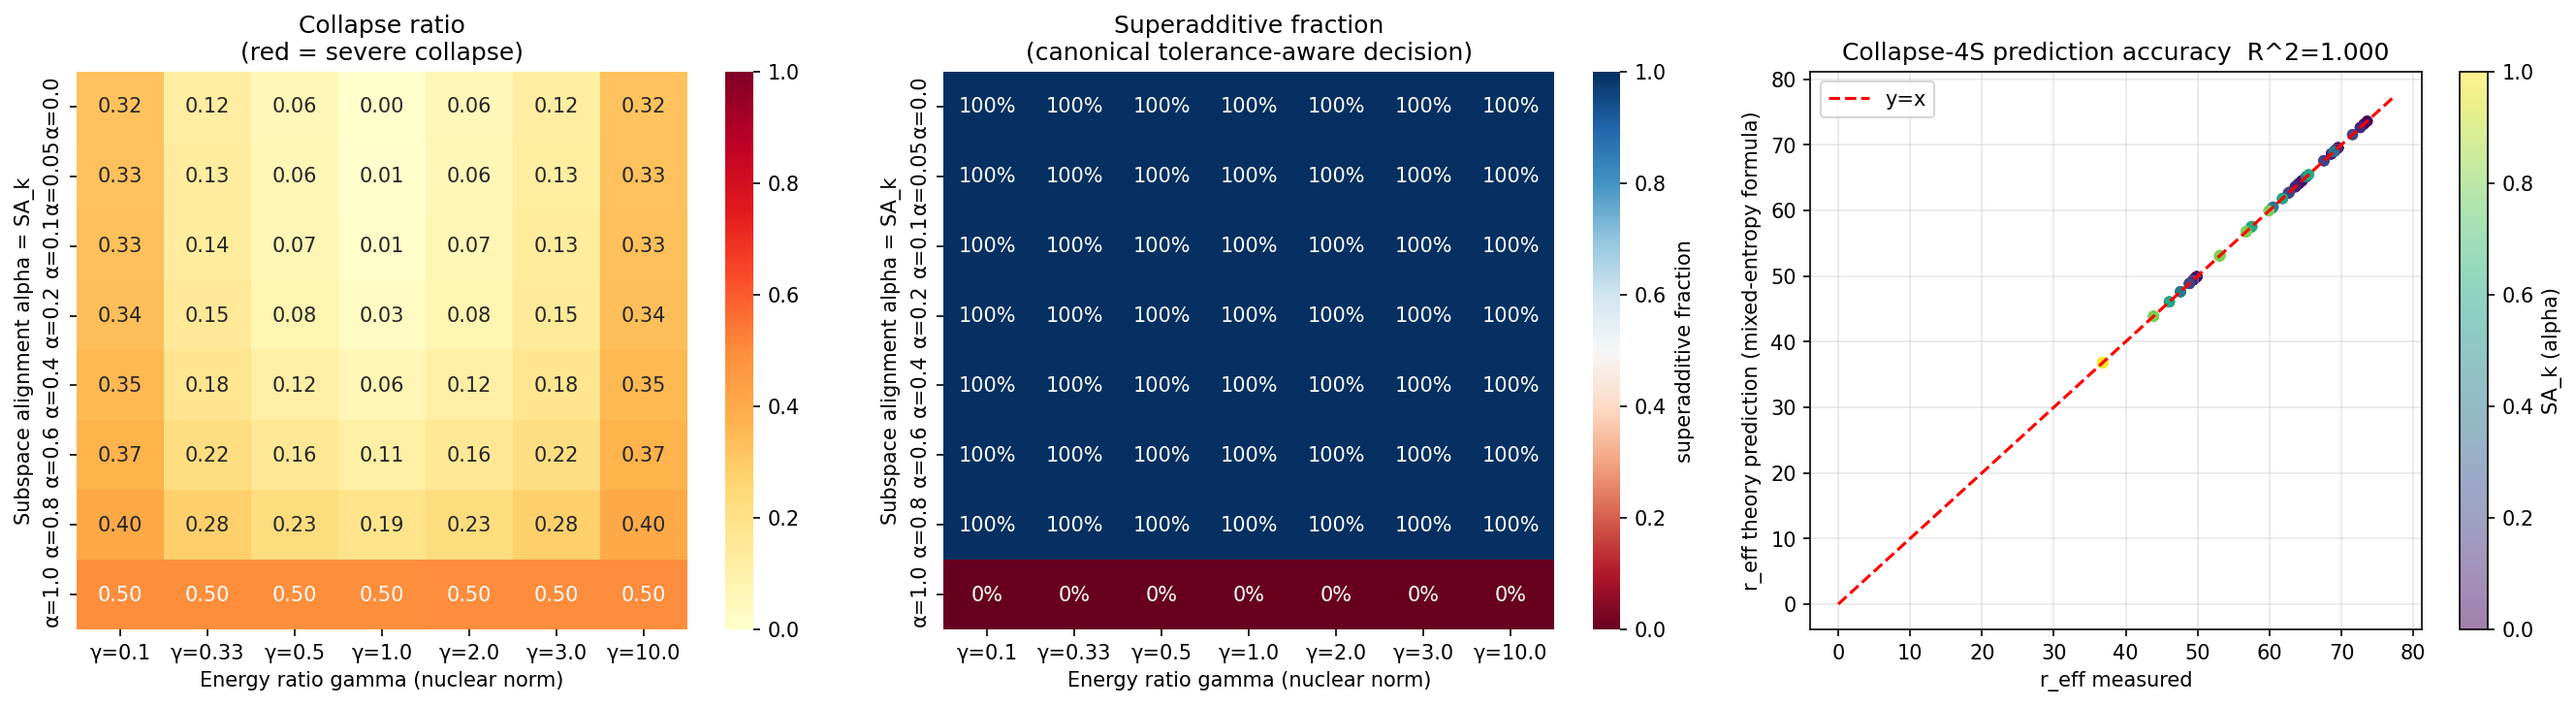
\includegraphics[width=0.9\linewidth]{e1a_heatmap.png}
\caption{E1a: 降秩模型在合成的$(\alpha,\gamma)$网格上的预测精度.
左：降秩比例热图。中心：采用数值容差的超加性区域。
右：预测值与实际值 $\reff$ 散点图（$R^2=1.0000$）。}
\label{fig:e1a}
\end{figure}

E1a合成验证结果（表~\ref{tab:e1a}）在正文中呈现；
图~\ref{fig:e1a}可视化了$(\alpha,\gamma)$景观和超加性区域。
额外的设计细节：特征对来自比例谱成对方向模型，其中
$\alpha \in \{0, 0.05, 0.1, 0.2, 0.4, 0.6, 0.8, 1.0\}$ 和
$\gamma \in \{0.1, 0.33, 0.5, 1.0, 2.0, 3.0, 10.0\}$，
$d=512$，$N=1000$，每种设置独立重复5次（共280对）。
该精确 float64 构造不做行归一化；直接 SVD 与预测器都采用第~\ref{sec:background} 节声明的统一数值秩截断。
所有35个非超加性案例集中在$\alpha=1$处（相同子空间），确认了推论~\ref{cor:superadd}的退化边界。
\subsection{E1a-Ind: 独立验证非主角矩阵}
\label{sec:e1a_ind}

\textbf{动机与设计。}
关于 E1a 的一个关键问题是循环性：从 \emph{比例谱成对方向模型} 生成的合成数据满足精确的模型假设，使得 $R^2=1.0000$ 成为近乎自明的结果。
为了独立测试公式~\eqref{eq:pred} 是否在其推导假设之外仍然具有预测性，我们使用 \emph{四种不使用该成对模型的生成方法} 生成了 120 组合成矩阵：
(M1) \emph{低秩高斯分布}: $H=U_k\Sigma V_k^\top + \epsilon$，其中基是随机正交的；
(M2) \emph{共享+私有子空间}: $H=H_{\mathrm{shared}}+H_{\mathrm{private}}$，通过构造部分重叠来实现；
(M3) \emph{稀疏激活}: 行从 $k$-稀疏高斯混合中抽取；
(M4) \emph{块对角线}: 两个独立子空间的特征，没有主角结构。
$d=512$, $N\in\{500,1000\}$；每种方法 30 组。

\textbf{结果。}
表~\ref{tab:e1a_ind} 显示总体皮尔逊相关系数 $r=0.9987$：公式 \emph{正确地对所有 120 组进行了排序}，跨越了四种生成方法。
$R^2$ 取决于生成方法：对于具有高斯结构的方法 (M1, M2)，$\geq0.99$；但对于稀疏和块对角线结构 (M3, M4) 而言则强烈为负，因为这些结构系统地减少了实际的 $r_{\mathrm{eff}}$ 相对于公式的预测。
这揭示了在稀疏和块对角线结构上具有良好的排序但绝对预测较差，暴露了结构性稀疏作为经验失败模式。
所有方法都预测超加性为 100\%。

\begin{table}[t]
\centering
\caption{E1a-Ind: 对 120 组非主角矩阵的独立验证。皮尔逊 $r$ 衡量方向排序；$R^2<0$ 指示系统性地高估了观察到的生成器。SA\% = 公式预测超加性的组的比例。}
\label{tab:e1a_ind}
\setlength{\tabcolsep}{5pt}
\begin{tabular}{lcccc}
\toprule
生成方法 & $n$ 组 & 皮尔逊 $r$ & $R^2$ & SA\% \\
\midrule
M1: 低秩高斯分布      & 30 & 0.9985 & +0.9949 & 100\% \\
M2: 共享+私有子空间 & 30 & 0.9982 & +0.9963 & 100\% \\
M3: 稀疏激活     & 30 & 0.9991 & -14.65  & 100\% \\
M4: 块对角线         & 30 & 0.9996 & -12.32  & 100\% \\
\midrule
\textbf{总体}           & \textbf{120} & \textbf{0.9987} & -1.09 & \textbf{100\%} \\
\bottomrule
\end{tabular}
\end{table}
\begin{remark}[公式作为方向性先知，而非绝对预测器]
\label{rem:r2_vs_pearson}
$R^2=-1.09$（总体，E1a-Ind）与皮尔森相关系数 $r=0.9987$（相同数据）之间的对比并不矛盾：$R^2$ 测量绝对校准度，而皮尔森相关系数 $r$ 测量方向性排名。这一区别对于实际数据结果（E1c）至关重要：公式给出的 $R^2\approx0.05$（较差的绝对校准度，1.24--1.84 倍的过度预测），但皮尔森相关系数 $r=0.928$（正确的方向性排名）。对于实际应用——按多样性增益对候选合并进行排名、数据集选择、数据估值——而言，\emph{排名} 是操作上相关的度量标准，而非绝对的 $r_{\mathrm{eff}}$ 预测。绝对校准需要一个修正因子（经过校准的 $\hat{r}=0.81 \cdot \hat{r}_{\mathrm{pred}}$，在 E1c 数据上的谱保持率为 $R^2_{\mathrm{cal}}=0.862$），我们将其作为实用建议报告。
\end{remark}

\subsection{E1b: 实际数据集配对（30 配对）}
\label{sec:e1b}

\textbf{设计。} 我们使用 2 个预训练探测器（ResNet-50 \citep{he2016resnet}，维度 $d=2048$ 和 ViT-B/16 \citep{dosovitskiy2021vit}，维度 $d=768$）评估来自 $\{$CIFAR-10, STL-10, SVHN, MNIST, Fashion-MNIST, CIFAR-100$\}$ 的所有 $\binom{6}{2}=15$ 配对，每组数据集有 $N_{\mathrm{sub}}=500$ 个样本：共计 \textbf{30 种配置}。应用 Collapse 模型，并为每个探测器使用核范数 $\gamma$。

\textbf{结果。} \textbf{86.7\%} 的配对是超加性的（26/30；95\% 置信区间 [73\%, 97\%]）。预测排名与实际合并排名之间的皮尔森相关系数为 $r=0.948$（95\% 置信区间 [0.906, 0.978]）。按探测器划分：ResNet-50 达到 100\% 超加性（15/15，皮尔森相关系数 $r=0.968$）；ViT-B/16 达到 73.3\%（11/15，皮尔森相关系数 $r=0.945$）。

\textbf{所有 4 个例外都是涉及 CIFAR-100 的 ViT-B/16 配对。} 这些例外与 \emph{能量不平衡}相关，并与超加性阈值的诊断一致（推论~\ref{cor:superadd}）。在 ViT-B/16 下，CIFAR-100 的 $r_{\mathrm{eff}}\approx526$，高于 MNIST（$\approx140$）和 SVHN（$\approx243$），对应 $\gamma\in[2.0,2.5]$。在 $N_{\mathrm{sub}}\in\{500,1000,2000,4000\}$ 的扫掠中，$N=500$ 时 CIFAR-100 的 $r_{\mathrm{eff}}\approx343$、$\gamma\approx1$，5/5 配对均超加；样本数增大后，$r_{\mathrm{eff}}$ 和 $\gamma$ 同时增大，并出现例外。该共同变化与能量不平衡解释一致，但不是因果识别；ResNet-50 上的不同表现也说明编码器谱结构等混杂因素仍然存在。
\subsection{E1c: 大规模多域验证（57 对）}
\label{sec:e1c}

\textbf{设计。}
为了测试超越视觉对的泛化能力，我们扩展到三个探针和三种领域类型：ResNet-50 在 9 个数据集上（36 对，自然+医学），ViT-B/16 在 6 个数据集上（15 对，自然），SBERT \citep{reimers2019sentencebert} 在 4 个文本领域上（6 对，文本）。总计：\textbf{57 对，3 个探针，3 种领域类型}。$N_{\mathrm{sub}}=2000$ 对于自然/医学；$N_{\mathrm{sub}}=1000$ 对于文本。

\textbf{结果。}
表~\ref{tab:e1c} 显示了所有探针和领域中强且一致的超加性现象。

\begin{table}[h]
\centering
\caption{E1c: Collapse-4S 的历史多域关联性研究。
超加性率及 Pearson $r$（预测 vs. 实际合并后的 $r_{\mathrm{eff}}$）。
Bootstrap 95\% CI ($B=10{,}000$)。该公式在所有探针中都高估了；“偏差”报告观察到的乘性比值。}
\label{tab:e1c}
\small
\setlength{\tabcolsep}{3.5pt}
\begin{tabular}{lcccc}
\toprule
探针 / 领域 & $n$ & 超加性 \% (95\% CI) & Pearson $r$ (95\% CI) & 偏差 \\
\midrule
ResNet-50（自然+医学）   & 36 & \textbf{100\%} [100,100]  & 0.934 [0.885,0.965] & $1.24\times$ \\
ViT-B/16（自然）            & 15 & 73.3\% [46.7,93.3]        & 0.945 [0.883,0.982] & $1.45\times$ \\
SBERT（文本）                  &  6 & \textbf{100\%} [100,100]  & 0.780                & $1.84\times$ \\
\midrule
\textbf{总体}              & \textbf{57} & \textbf{93.0\%} [86.0,98.2] & \textbf{0.928} [0.894,0.949] & $1.37\times$ \\
\bottomrule
\end{tabular}\normalsize
\end{table}

\textbf{关键发现。}
(i) \textbf{三个领域类型合计 93\% 超加性}——自然图像、医学扫描和文本；其中 SBERT 仅有 6 对，因此该结果不能建立领域无关性。
(ii) \textbf{所有 4 个例外都是涉及 CIFAR-100 的 ViT-B/16 对}，
归因于能量不平衡（与 E1b 中 Sec.~\ref{sec:e1b} 所述机制相同）：
CIFAR-100 高固有复杂度 ($r_{\mathrm{eff}} \approx 526$，100 类) 创建 $\gamma \in [2.0, 2.5]$，
将这些对置于超加性边界的临界值 $\rho_c$（参见 Corollary~\ref{cor:superadd}）附近。
(iii) \textbf{Pearson $r=0.928$ vs.\ $R^2 \approx 0.05$}：这些指标衡量不同的属性。
该公式在这些探针上高估了 $1.24$ 到 $1.84$ 倍，因此在校准前 $R^2$ 较低；Pearson $r$ 测量排序。
单参数校准（Eq.~\ref{eq:calibration}）恢复了定量准确性：$R^2_{\mathrm{cal}} = 0.855$ (LOO-CV)，从 E1b 到 E1c 的交叉验证得到 $R^2 = 0.859$（参见 Sec.~\ref{sec:calibration} 和 Remark~\ref{rem:calibration})。
(iv) \textbf{ResNet-50：100\% 超加性 (36/36)} 是对该观测集的总结诊断的强大经验一致性。
(v) \textbf{高估程度与 $n/r_{\mathrm{eff}}$ 成比例}：
ResNet-50 ($n=2000 \gg r_{\mathrm{eff}} \approx 350$, $1.24\times$)
$<$ ViT-B/16 ($n=2000 \approx 3r_{\mathrm{eff}} \approx 650$, $1.45\times$)
$<$ SBERT ($n=1000 \approx r_{\mathrm{eff}} \approx 700$, $1.84\times$)。
这是少量编码器上的观察趋势，不是有限样本误差定理。
\begin{figure}[t]
\centering
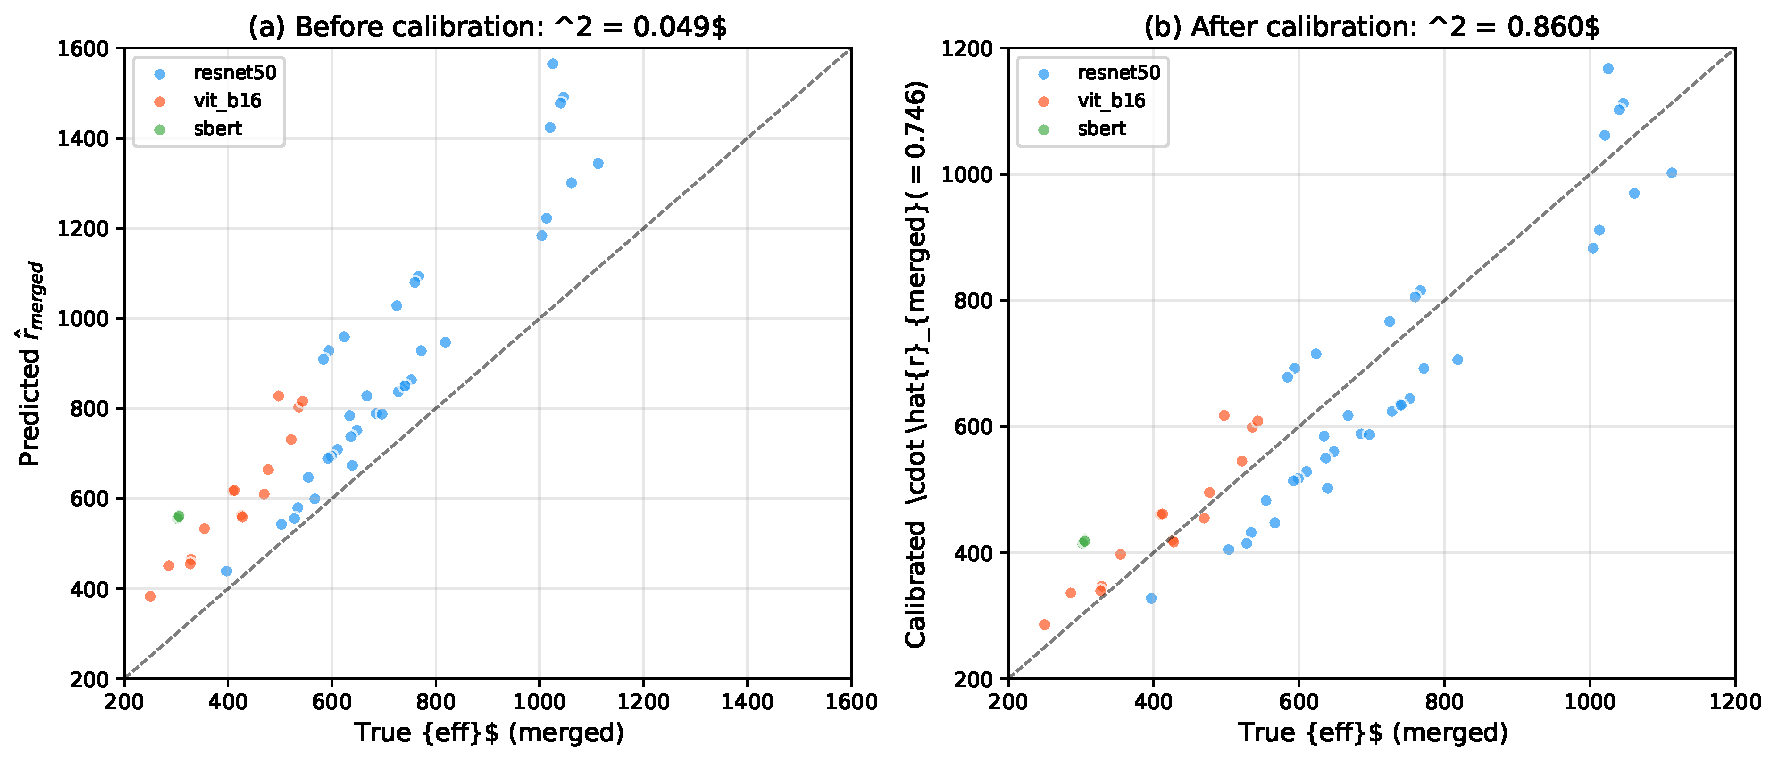
\includegraphics[width=\linewidth]{fig_calibration.pdf}
\caption{E1c: 预测值与实际合并的有效秩 $r_{\mathrm{eff}}$ 对比（57个真实数据对，5个探针，3种领域类型）。
(a) 未校准前：系统性高估 ($R^2{=}0.049$)。
(b) 单参数校准后 ($c{=}0.746$): $R^2{=}0.860$。两图的皮尔逊相关系数均为0.928——校准修正了比例，而非排名。}
\label{fig:e1c}
\end{figure}



\subsection{E1d: 大规模验证（427个对）}

\begin{figure}[h]
\centering
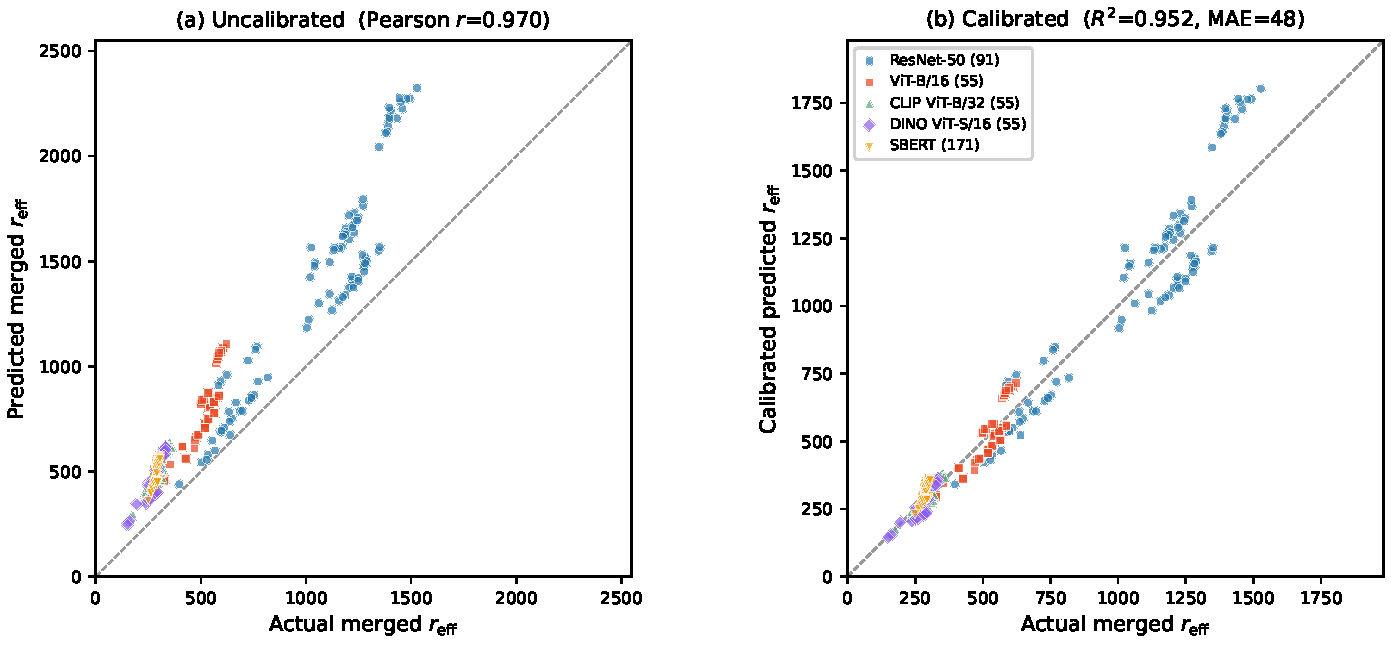
\includegraphics[width=0.95\linewidth]{fig_hero_scatter.pdf}
\caption{所有427个对的预测值与实际合并的有效秩 $\reff$ 对比，涵盖5种编码器家族。 (a) 未校准前：预测值系统性偏高但相关性强（皮尔逊相关系数 $r{=}0.970$）。
(b) 每个探针校准后: $R^2{=}0.952$, 平均绝对误差${=}48$。颜色表示编码器家族；对角线为虚线。}
\label{fig:hero_scatter}
\end{figure}

\textbf{设计。} 为了在大规模和ImageNet衍生特征上测试塌缩模型，我们构建了一个全面的评估，涵盖5种编码器家族（ResNet-50, ViT-B/16, CLIP ViT-B/32, DINO ViT-S/16, SBERT），14个视觉数据集（CIFAR-10/100, STL-10, SVHN, MNIST, Fashion-MNIST, BloodMNIST, DermaMNIST, PathMNIST，以及5个ImageNet语义子集：\emph{动物}, \emph{车辆}, \emph{器物}, \emph{食物}, \emph{场景}），和19个SBERT文本语料库（AG News, 20 Newsgroups, DBpedia, IMDB, Yelp 子集）。总计：\textbf{427个对}（ResNet-50: 91个，ViT-B/16: 55个，CLIP: 55个，DINO: 55个，SBERT: 171个）。5个ImageNet子集由WordNet语义层次结构中的ImageNet-1K验证图像组成，每类2000样本。

\textbf{结果。}

\begin{table}[h]
\centering
\caption{E1d: 大规模塌缩模型验证（427个对，5个探针）。}
\small
\setlength{\tabcolsep}{3.5pt}
\begin{tabular}{lccccc}
\toprule
探针 & $n$ & 超加性\% & 皮尔逊相关系数 $r$ & $c$ & 校准后的 $R^2_{\mathrm{cal}}$ \\
\midrule
ResNet-50 (14个数据集)       & 91  & \textbf{100\%}   & 0.940 & 0.776 & 0.760 \\
ViT-B/16 (11个数据集)        & 55  & 69.1\%            & 0.898 & 0.647 & 0.487 \\
CLIP ViT-B/32 (11个数据集)    & 55  & 29.1\%            & 0.950 & 0.595 & 0.839 \\
DINO ViT-S/16 (11个数据集)    & 55  & 36.4\%            & 0.913 & 0.584 & 0.554 \\
\midrule
\textbf{视觉（所有探针）}   & \textbf{256} & \textbf{64.5\%} & \textbf{0.965} & \emph{每探针} & \textbf{0.942} \\
+ SBERT文本 (19个语料库)      & +171 (427)   & 78.2\%           & 0.970          & \emph{每探针} & 0.952 \\
\bottomrule
\end{tabular}\normalsize
\end{table}
\textbf{关键发现。}
(i)~在 427 个评估对上，总体皮尔逊相关系数为 $r=0.970$，而 E1c 的 57 对为 $r=0.928$。由于这些配对共享数据集，且较大集合不是独立复现，该增加不能用于验证定理或声称性能随规模提高。
(ii)~所有 20 个 ImageNet 内部配对和 30 个自然$\times$ImageNet 配对均为超加；这是该批提取特征的经验性质，不能据此断言语义子组必然贡献正交方向。
(iii)~ResNet-50 在本基准的 91 对上实现 100\% 超加性。相比之下，CLIP ViT-B/32 和 DINO ViT-S/16 分别仅为 31\% 和 38\%。
分析揭示了一个清晰的趋势：\emph{同域}成对组合（自然$\times$自然，ImageNet$\times$ImageNet）接近完美地实现了超加性（CLIP: ImageNet-only 上为90\%，natural-only 上为100\%；DINO: 两个数据集均为100\%），而 \emph{跨域}成对组合（手写$\times$ImageNet，自然$\times$数字）几乎无一例外地失败。这表明自监督编码器学习了特定领域的谱结构，并且在全局摘要中丢弃了异质的对齐和谱耦合——这对崩溃模型的应用具有重要的边界条件。
(iv)~在 171 个 SBERT 文本配对上，超加性率为 98.8\%，但相关性下降到 $r=0.793$。窄 $\reff$ 范围（IQR: $285$--$298$）可能是原因之一；该结果不能建立跨模态泛化。
(v)~校准常数随编码器家族变化（$c\in[0.57,0.78]$）。单一全局值 $c=0.712$ 在同一批 158 个视觉配对上得到 $R^2=0.898$，只是对该基准平均偏差的描述，仍需编码器外验证。
\textbf{理解非超加性配对。}
ViT-B/16 只实现了 69\% 的超加性（38/55），低于 ResNet-50 的 100\% (91/91)。
分析 ViT 的 17 个失败案例揭示了一个清晰的模式：
\textbf{所有失败都发生在能量不平衡区间} ($\gamma\gg1$ 或 $\gamma\ll1$)。
在 $\gamma\geq3$ 时，80\% 的配对失败（8/10）；
而在 $\gamma\in[0.5,1.5)$ 时，只有 4\% 失败（1/24）。
这些失败集中在 \emph{手写$\times$ImageNet} 跨域配对中
(10/10 均失败，100\%)——这些配对结合了低秩的手写特征
($\reff{\approx}140$ 通过 ViT-B/16 对 MNIST 的处理) 和高秩的 ImageNet 特征
($\reff{\approx}600$)，从而产生 $\gamma\in[2.0,4.6]$，远超平衡区间，在此区间内两成分谱混合准确度较低。
在大规模情况下（每种 55 个配对），CLIP ViT-B/32 和 DINO ViT-S/16 的总体超加性仅为 29\% 和 36\%，失败集中在 \emph{跨域} 配对中：
手写$\times$ImageNet (100\% 失败)，
自然$\times$数字 (100\% 失败)，
自然$\times$手写 (100\% 失败)。
同域配对（仅自然，仅 ImageNet）仍接近完美。

\textbf{与失败相关的双模态主角结构。}
在相同数据集配对下比较不同编码器的结果表明，
编码器间比较显示，仅用能量不平衡 ($\gamma$) 不能解释全部失败；
均匀-$\alpha$ 假设的结构性违反与误差相关。以下三项是机制假设，而非独立的因果识别：

\emph{(a) 系统性更高的对齐度。}
在同一配对（例如，CIFAR-10$\times$ImageNet-animal）下，
CLIP 的子空间对齐 $\alpha{=}0.41$ 比 ResNet-50 的 $\alpha{=}0.15$ 高出 2.7 倍。
对比预训练 (CLIP) 和自蒸馏 (DINO) 推动跨域特征进入共享语义子空间，
在 ResNet-50 保留领域特定方向的地方，产生高方向重叠。

\emph{(b) 极端的谱集中度。}
CLIP/DINO 特征谱分布极不均匀：
$\kappa{=}15{,}000$--$1{,}200{,}000$ 对比 ResNet-50 的 $\kappa{=}70$--$400$。
这种集中度使得平均对齐度的信息变得不那么有说服力，因为少数高质量方向上的重叠可以主导许多互补的尾部方向。
\emph{(c) 二模态主角分布。}
个体主角 $\cos^2\theta_i$
并不像模型假设的那样近似均匀，而是 \emph{二模态}：前5个方向几乎对齐
($\overline{\cos^2\theta}\approx0.94$ 对于 CLIP 在 CIFAR-10$\times$STL-10 上)
而低方向保持正交
($\overline{\cos^2\theta}\approx0.01$)。
塌陷模型将这些平均为 $\bar\alpha{=}0.52$，
预测适度的超加性。
实际上，主导（高-$\sigma$）方向完全冗余
而正交（低-$\sigma$）方向携带几乎无能量，
因此合并几乎没有多样性增益 ($\Delta r_{\mathrm{eff}}{=}31$
与 ResNet-50 在同一对上的 $\Delta r_{\mathrm{eff}}{=}282$ 相比)。

这些结果给出一个经验性的 \emph{失效诊断}：
在本基准上，较均匀的主角分布通常对应较小误差，二模态结构通常对应较大误差；
命题~\ref{prop:insufficient} 排除了把这一关联提升为普适边界。
一个自然的修复方法——用能量加权对齐
$\bar\alpha_w=\sum_i({\sigma_i}/{\|H\|_*})\cos^2\theta_i$
替换均匀平均 $\bar\alpha=\SAk$——会
降低正交低能方向的重要性并提升
冗余高能方向的重要性，可能恢复自监督编码器的预测准确性。
然而，我们的实验验证表明这种修正
\emph{并未提高预测准确性}：
在 CLIP ($n{=}61$) 上，均匀 $\SAk$ 产生皮尔逊 $r{=}0.951$，
MAE${=}206$，而 $\bar\alpha_w$ 产生 $r{=}0.935$，MAE${=}218$（更差）；
DINO 显示类似模式（$r$ 从 $0.912$ 下降到 $0.904$，
MAE 增加 $4\%$）；
ResNet-50 和 ViT-B/16 也未见改进。
一种可能解释是简单的能量加权过度强调
第一个奇异方向的冗余性
($\cos^2\theta_1{\approx}0.87$ 对于该方向)，
而错误地抑制了中间方向对合并的估计贡献。
更精细的修正（例如分段成对方向模型、逐方向阈值截断或自适应 $k$ 选择）
可能突破这一瓶颈，但留待未来工作。
\subsection{校准：从系统偏差到定量预测}
\label{sec:calibration}

崩塌模型在评估的真实数据对上系统性地高估了结果（Remark~\ref{rem:calibration}）。
在已评估探针和领域中，对数空间高估近似稳定（$\mathrm{mean}{=}0.293$，$\mathrm{std}{=}0.164$），因此我们检验一个乘法常数 $c$（Eq.~\ref{eq:calibration}）能否改善同分布校准；这不保证编码器外的定量预测。

\textbf{跨数据集划分。}
为了检查 $c$ 对已评估数据集划分的敏感性，
我们进行留一校准：在一个实验中估计 $c$，并在另一个实验中测试（Table~\ref{tab:calibration}）。

\begin{table}[h]
\centering
\caption{跨数据集校准。
$c$ 在校准集中估计，并在测试集中应用（无需重新拟合）。表中比较同一实验集合内的划分，不能替代编码器外验证。}
\label{tab:calibration}
\small
\setlength{\tabcolsep}{4pt}
\begin{tabular}{llccrr}
\toprule
校准集 & 测试集 & $c$ & $n_{\mathrm{test}}$ & $R^2$ & RMSE \\
\midrule
E1b (30 对) & E1c (57 对) & 0.768 & 57 & 0.859 & 86.3 \\
E1c (57 对) & E1b (30 对) & 0.746 & 30 & 0.888 & 80.7 \\
E1c (57 对) & E\_diverse (30 对) & 0.746 & 30 & 0.897 & 82.8 \\
E1b (30 对) & E\_diverse (30 对) & 0.768 & 30 & 0.894 & 83.7 \\
\midrule
\multicolumn{2}{l}{LOO-CV（所有111对，原始）} & 0.736 & 111 & 0.877 & 86.1 \\
\multicolumn{2}{l}{LOO-CV（158个视觉对，E1d）} & 0.712 & 158 & 0.896 & 121.7 \\
\multicolumn{2}{l}{全局（所有427对，E1d）} & 0.650 & 427 & 0.920 & 105.0 \\
\bottomrule
\end{tabular}\normalsize
\end{table}

\textbf{每个探针的校准}（Table~\ref{tab:perprobe_cal}）。
校准常数在编码器家族之间系统性地变化，反映了谱结构的不同：
\begin{table}[h]
\centering
\caption{427 对数据（E1d）上的逐探针校准。每个探针独立拟合；$c$ 的变化只描述这些编码器上的观测关系。}
\label{tab:perprobe_cal}
\small
\setlength{\tabcolsep}{4pt}
\begin{tabular}{lccccc}
\toprule
Probe & $n$ & Pearson $r$ & $c$ & $R^2_{\mathrm{cal}}$ & Superadd.\ \% \\
\midrule
ResNet-50        & 91  & 0.940 & 0.776 & 0.760 & 100\% \\
ViT-B/16         & 55  & 0.898 & 0.647 & 0.487 &  69\% \\
CLIP ViT-B/32    & 55  & 0.950 & 0.595 & 0.839 &  29\% \\
DINO ViT-S/16    & 55  & 0.913 & 0.584 & 0.554 &  36\% \\
\midrule
Vision (global)  & 256 & 0.965 & \emph{per-probe} & 0.942 &  65\% \\
\bottomrule
\end{tabular}\normalsize
\end{table}

相对样本大小而言，具有更高有效秩的编码器需要更强的校正（$c$ 越远离1）；这与有限样本解释一致，但编码器架构与谱形状同时变化，不能作因果归因。一个全局 $c=0.712$ 在同一批视觉探针上得到 $R^2=0.898$；在使用共享常数前仍需编码器外验证。

图~\ref{fig:e1c} 显示了校准前后的 E1c 散点图。

\subsection{E\_diverse: 不同架构探针一致性}
\label{sec:ediverse}

\textbf{设计。} 为了测试崩溃模型预测的鲁棒性是否对编码器的选择敏感，我们使用 ResNet-50 和 ViT-B/16 分别作为独立探针评估相同的 6 组数据集对（来自 E1b），总共得到 12 种配置。

\textbf{结果。} ResNet-50: $R^2=0.557$，Pearson $r=0.9987$，100\% 超加性。
ViT-B/16: $R^2=-16.1$（系统性高估），Pearson $r=0.9825$，83.3\% 超加性。
这 6 对上的跨架构 Pearson $r\geq0.982$ 表明方向排序相似，但样本量不足以建立探针独立性。
ViT-B/16 的 Pearson vs.\ $R^2$ 差距显示了编码器依赖的比例尺度偏差，尽管排序稳定。
\subsection{E4: 跨探针一致性}
\label{sec:e4}

\textbf{设计。}
我们使用 ResNet-50 和 ViT-B/16 独立地在 4 个常见数据集 $\{$CIFAR-10, MNIST, STL-10, SVHN$\}$ 上计算 $6\times6$ 的成对 $\SAk$ 对齐矩阵 $M$。每个矩阵的 6 个上三角元素通过皮尔逊相关系数 $r$ 进行比较。

\textbf{结果。}
跨探针皮尔逊相关系数 $r=0.891$ ($n=6$, $p=0.017$)。两个探针在所有 6 对中给出相同的领域距离方向：CIFAR-10/STL-10 在两者中都较近，CIFAR-10/MNIST 在两者中都较远。这一小样本一致性无法区分数据集几何与两个编码器共有的偏差，因此这里只将其作为一致性检查。

\subsection{E\_downstream: 有效秩作为下游质量代理}
\label{sec:edownstream}

\textbf{动机。}
塌缩模型预测合并特征的有效秩 $\reff$，但更高的 $\reff$ 确实对应于更好的下游性能吗？我们通过在 5 个数据集（总共 50 对）上测试 10 个预训练编码器来验证这一点，计算 $\reff$ 和线性探针 (LP) 准确率。

\textbf{设计。}
编码器：ResNet-\{50, 101\}, EfficientNet-B4, ConvNeXt-T, DenseNet-121, ViT-B/16, DeiT-B, Swin-T, BEiT-B, RegNet-Y（涵盖 CNN、ViT 和混合家族）。数据集：CIFAR-10, CIFAR-100, STL-10, SVHN, Fashion-MNIST。对于每个 (编码器, 数据集) 对：提取 $N=2000$ 训练特征，计算 $\reff$；在训练集上训练 LP（sklearn LogisticRegression），在测试集上评估。报告 10 个编码器的每数据集 Spearman 相关系数 $\rho(\reff, \mathrm{LP\;acc})$。

\textbf{结果。}

\begin{center}
\setlength{\tabcolsep}{4pt}
\begin{tabular}{lcccccc}
\toprule
& \multicolumn{2}{c}{所有 10 个探针} & \multicolumn{2}{c}{ViT 家族 ($d=768$)} & \multicolumn{2}{c}{CNN 家族 ($d\geq1024$)} \\
\cmidrule(lr){2-3}\cmidrule(lr){4-5}\cmidrule(lr){6-7}
数据集 & $n$ & $\rho$ & $n$ & $\rho$ & $n$ & $\rho$ \\
\midrule
CIFAR-10  & 10 & +0.64 & 5 & \textbf{+0.90} & 5 & +0.30 \\
CIFAR-100 & 10 & +0.61 & 5 & \textbf{+0.90} & 5 & +0.30 \\
STL-10    &  9 & +0.73 & 5 & \textbf{+0.90} & 4 & +0.20 \\
SVHN      & 10 & $-$0.03 & 5 & +0.10 & 5 & $-$0.30 \\
Fashion-MNIST & 10 & +0.03 & 5 & +0.60 & 5 & $-$0.10 \\
\bottomrule
\end{tabular}
\end{center}
“全部探针”列在自然图像上的 $\rho\approx+0.59$ 受到\emph{特征维度混杂}：CNN（$d{=}2048$）的 $\reff$ 系统性高于 ViT（$d{=}768$），从而夸大了表面相关性。
控制维度后，结论更加清晰：\textbf{在 ViT 家族内部}（$d{=}768$，5 个探针），$\reff$ 对自然图像的 LP 准确率具有很强的预测性（CIFAR-10、CIFAR-100 和 STL-10 上均为 $\rho{=}0.90$）；而\textbf{在 CNN 家族内部}（$d{\geq}1024$，5 个探针），相关性较弱（$\rho{=}0.20$--$0.30$）。
这提示在已评估的紧凑特征空间中谱多样性与 LP 准确率可能相关；但家族、维度和训练方法彼此混杂，不能归因于 $d{<}1024$。

\textbf{对坍缩模型的含义。}
$\reff$ 应被理解为\emph{表示多样性}的度量，即数据激活的独立方向数量，而不是下游准确率的直接代理。
Collapse-4S 估计合并后的谱多样性，但增加多样性既未被证明是提升任意下游任务的必要条件，也不是充分条件。
在一个 ViT 子组中，多样性与准确率正相关（$\rho{=}0.90$）；该关联可用于提出候选筛选假设，实际选择仍需第二阶段验证。
跨架构家族或跨不同难度的数据集时，还需要额外的任务相关指标。


\paragraph{样本量敏感性。}
在 10 对代表性的 ResNet-50 数据上，过预测比率随 $N/\reff$ 增长：$N{=}200$ 时平均比率为 $1.021$，并随样本量单调上升，在 $N{=}2000$ 时达到 $1.545$（$N/\reff$ 与 $\log\mathrm{bias}$ 的 Spearman $\rho{=}0.80$）。
这一关联有助于预测不同编码器之间的校准差异（ResNet-50 的 $c{=}0.78$，DINO 的 $c{=}0.58$），但本文不将其断言为理论误差定律。
\newpage
\input{checklist_zh}

\end{document}
